%%%%%%%%%%%%%%%%%%%%%%%%%%%%%%%%%%%%%%%%%%%%%%%%%%%%%%%%%%%%%%%%%%%%%%
% Lớp 11 | Đường thẳng, mặt phẳng. Quan hệ song song trong | Hai đường thẳng song song
% Dạng 1H4?2-5: Xác định thiết diện bằng cách kẻ song song
% Số câu: 50  (sinh tự động bởi tach_cau.py; từ nay thầy sửa trực tiếp file này)
%%%%%%%%%%%%%%%%%%%%%%%%%%%%%%%%%%%%%%%%%%%%%%%%%%%%%%%%%%%%%%%%%%%%%%

%%%%%%%%%%%%%%%% TRẮC NGHIỆM 4 PHƯƠNG ÁN %%%%%%%%%%%%%%%%

% nguồn: Ok_Toan11_TracNghiem_Lan2
\begin{ex}%[1H4H2-5]%[ma:980cb988]
	Cho tứ diện $ABCD$. Gọi $M$, $N$ lần lượt là trung điểm các cạnh $AB$ và $AC$, $E$ là điểm  trên cạnh $CD$ với $ED=3EC$. Thiết diện tạo bởi mặt phẳng $(MNE)$ và tứ diện $ABCD$ là
	\choice 
		 {Tam giác $MNE$}
		{Tứ giác $MNEF$ với $F$ là điểm bất kì trên cạnh $BD$} 
		{Hình bình hành $MNEF$ với $F$ là điểm trên cạnh $BD$ mà $EF\parallel BC$} 
		{\True Hình thang $MNEF$ với $F$  là điểm trên cạnh $BD$ mà $EF\parallel BC$}
	 \loigiai{
	 \immini
		{ 
		Tam giác $ABC$ có $M$, $N$ lần lượt là trung điểm  của $AB, AC$.\\
		 Suy ra $MN$ là đường trung bình của tam giác $ABC\Rightarrow MN\parallel BC$.\\
		Từ $E$ kẻ đường thẳng $d$ song song với $BC$ và cắt $BD$ tại  $F\Rightarrow EF\parallel BC$.\\
		Do đó $MN\parallel EF$ suy  ra bốn điểm $M$, $N$, $E$, $F$ đồng phẳng và $MNEF$ là hình thang.\\
		Vậy hình thang $MNEF$ là  thiết diện cần tìm.
		 }
		{ 
		\begin{tikzpicture}[scale=0.8,font=\footnotesize,line join=round,line cap=round,>=stealth]
				 \def\h{2.5}
				\path (0,0) coordinate (B)--(4,0) coordinate (C)--(1.5,-1.5) coordinate  (D)--($(B)+(1,\h)$) coordinate (A);
				\coordinate (M) at  ($(A)!0.5!(B)$);
				\coordinate (N) at  ($(A)!0.5!(C)$);
				\coordinate (E) at ($(C)!1/4!(D)$); 
				\coordinate (f) at  ($(E)+(M)-(N)$);
				\coordinate (F) at (intersection of E--f and B--D); 
				\fill[pattern=north  east lines,opacity=0.5] (M)--(N)--(E)--(F)--cycle;
				 \draw (D)--(B)--(A)--(C)--cycle (A)--(D)
					(M)--(F) 
					(N)--(E); 
				\draw[dashed] (B)--(C) 
					 (M)--(N)
					 (E)--(F);
				\foreach \x/\g in {A/90,B/180,C/0,D/-90,M/150,N/40,E/-30,F/220}\fill (\x)  circle (1pt)+(\g:0.25) node{$\x$};
			\end{tikzpicture}
		 }
	} 
\end{ex}

% nguồn: Ok_Toan11_TracNghiem_Lan2
\begin{ex}%[1H4H2-5]%[ma:b0eb417b]
	Cho hình lập phương $ ABCD.A'B'C'D'$, $ AC\cap BD=O$, $ A'C'\cap B'D'=O'$. Gọi $ M$, $ N$, $ P$ lần lượt là trung điểm các cạnh $ AD$, $ DC$, $ CC'$. Khi đó thiết diện do mặt phẳng $\left(MNP\right)$ cắt hình lập phương  là hình:
	 \choice
		 {Tam giác}
		{Tứ giác} 
		 {Ngũ giác}
		{\True Lục  giác}
	 \loigiai{
		\begin{center}
			\begin{tikzpicture}[declare function={goc=225; a=3; b=5; h=5;},scale=0.8]
					 \path
						(0,0)  coordinate (B)--+(0,h) coordinate (B')
						(b,0)  coordinate (C)--+(0,h) coordinate (C')
						 (goc:a) coordinate (A)--+(0,h) coordinate (A')
						($(A)+(C)-(B)$) coordinate (D)--+(0,h)  coordinate (D')
						($(A)!.5!(D)$) coordinate  (M)
						 ($(D)!.5!(C)$) coordinate (N)
						($(C)!.5!(C')$) coordinate (P) 
						($(B')!.5!(C')$) coordinate (Q) 
						 ($(A')!.5!(B')$) coordinate (R)
						($(A)!.5!(A')$) coordinate (S) 
						(intersection of A--C  and B--D) coordinate (O)
						 (intersection of A'--C' and B'--D') coordinate (O');
					\fill  [green!30] (M)--(N)--(P)--(Q)--(R)--(S)--cycle;
					\draw[dashed] (B)--(B') 
						 (A)--(B)--(C)
						(M)--(N) 
						(S)--(R) 
						 (Q)--(P)
						 (A)--(C)
						(B)--(D); 
					\draw (A')--(B')--(C')--(D')--cycle (A)--(A') 
						 (D)--(D')
						 (C)--(C')
						 (A)--(D)--(C)
						 (S)--(M)
						 (R)--(Q)
						(N)--(P) 
						 (A')--(C')
						 (B')--(D');
					\foreach \x/\g in {A/180,B/180,C/0,D/-30,A'/90,B'/90,C'/-15,D'/90,M/-90,N/0,P/0,R/90,S/180,Q/90,O/0,O'/-90}{ 
						 \draw[fill=black] (\x) circle (1pt) node[shift={(\g:7pt)},font=\footnotesize]{$\x$};}
				\end{tikzpicture}
		\end{center}
		Ta có $\left\{\begin{array}{l}
		MN\parallel AC\\ 
		NP\parallel  AB'.
	\end{array}\right.\Rightarrow\left(MNP\right)\parallel\left(AB'C\right)$\\
	$\Rightarrow\left(MNP\right)$ cắt hình lập phương  theo thiết diện là lục giác.
	 }
\end{ex}

% nguồn: Ok_Toan11_TracNghiem_Lan2
\begin{ex}%[1H4H2-5]%[ma:abf5b330]
	Cho hình chóp $S.ABCD$, có đáy $ABCD$ là hình bình hành. Gọi $M$ là trung điểm của $SD$, $N$  là điểm trên cạnh $SB$ sao cho $SN=2SB$, $O$ là giao điểm của $AC$ và $BD$. Khẳng định nào sau đây \textbf{sai}?
	 \choice
		{Đường thẳng $MN$ cắt mặt phẳng  $\left(ABCD\right)$}
		{\True  Thiết diện của hình chóp $S.ABCD$ với mặt phẳng $\left(AMN\right)$ là một hình thang}
		{Hai đường thẳng $MN$ và $SO$  cắt nhau}
		{Hai đường thẳng $MN$  và $SC$ chéo nhau}
	 \loigiai{
		\begin{center}
			\begin{tikzpicture}[declare function={gocx=80; goc=-150; a=4.5; b=a/2; h=5;}]
					\path (0,0) coordinate (A)--+(gocx:h) coordinate (S) 
						 (a,0) coordinate (B)
						(goc:b)  coordinate (D)
						 +(a,0) coordinate (C)
						($(S)!.5!(D)$)  coordinate (M)
						 ($(S)!2/3!(B)$) coordinate (N)
						(intersection of A--C and B--D) coordinate (O) 
						(intersection of  S--O and M--N) coordinate (I)
						(intersection of A--I  and S--C) coordinate (K);
					\draw[dashed] (S)--(A) 
						(D)--(A)--(B) 
						 (A)--(N)--(M)--(A)
						 (A)--(C)
						 (B)--(D)
						(S)--(O) 
						(A)--(K); 
					\draw (S)--(D)--(C)--(S)--(B)--(C)--cycle  (M)--(K)--(N);
					\foreach  \x/\goc in {S/90,A/150,B/0,C/-60,D/-180,M/180,N/0,O/-90,I/30,K/30}
					\draw[fill=black]  (\x) node[shift={(\goc:7pt)},font=\scriptsize]{$\x$} circle (1pt);
				\end{tikzpicture}
		\end{center}
		$MN\cap BD=I\Rightarrow  MN\cap\left(ABCD\right)=I.$ nên A đúng.\\
		Hai đường  thẳng $MN$ và $SO$ cắt nhau do cùng nằm trong mặt phẳng $\left(SBD\right)$ và không song song nên C đúng.\\
		Hai đường thẳng $MN$ và $SC$ chéo nhau vì không cùng nằm trong một mặt phẳng nên D  đúng.
	 }
\end{ex}

% nguồn: Ok_Toan11_TracNghiem_Lan2
\begin{ex}%[1H4H2-5]%[ma:9ac38bbb]
	Cho hình chóp $ S.ABCD$ có đáy $ABCD$ là hình bình hành tâm $O$. Gọi $M$ là trung điểm của $ OB$, $\left(\alpha\right)$ là mặt phẳng đi qua $ M$, song song với $ AC$ và song song với $SB$. Thiết diện của hình chóp $S.ABCD$ khi cắt bởi mặt  phẳng $\left(\alpha\right)$ là hình gì?
	 \choice
		{Lục giác} 
		 {\True Ngũ giác}
		{Tam giác} 
		 {Tứ giác}
	 \loigiai{
		\begin{center}
			\begin{tikzpicture}[declare function={gocx=80; goc=-150; a=4.5; b=a/2; h=5;}]
					\path (0,0) coordinate (A)--+(gocx:h)  coordinate (S)
						 (a,0) coordinate (B)
						(goc:b) coordinate  (D)
						+(a,0) coordinate  (C)
						(intersection of A--C and B--D) coordinate (O) 
						($(O)!.5!(B)$) coordinate (M) 
						($(A)!.5!(B)$) coordinate (I) 
						($(C)!.5!(B)$) coordinate  (H)
						($(S)!.5!(A)$)  coordinate (J)
						 ($(S)!.5!(C)$) coordinate (L)
						($(D)!3/4!(S)$) coordinate  (K);
					\draw[dashed] (S)--(A) 
						 (D)--(A)--(B)
						 (A)--(C)
						 (B)--(D)
						(J)--(I)--(H) 
						(L)--(K)--(J) 
						 (M)--(K);
					\draw  (S)--(D)--(C)--(S)--(B)--(C)--cycle (H)--(L);
					\foreach \x/\goc  in {S/90,A/150,B/0,C/-60,D/-180,M/-90,O/-90,I/220,H/0,J/180,L/45,K/180}
					\draw[fill=black] (\x) node[shift={(\goc:7pt)},font=\scriptsize]{$\x$} circle  (1pt);
				\end{tikzpicture}
		\end{center}
		Ta  có:\\
		$\left\{\begin{array}{l}
		M\in\left(\alpha\right)\cap\left(ABCD\right)\\ 
		 \left(ABCD\right)\supset AC\parallel\left(\alpha\right)
	\end{array}\right.\Rightarrow\left(\alpha\right)\cap\left(ABCD\right)=d_1$ đi qua $ M$ và song song với $ AC$.\\
	Trong $\left(ABCD\right)$, gọi $ I,H$ lần lượt là giao điểm của $d_1$ với $ AB$ và $ BC$. Khi đó, $ I$ và $ H$ lần lượt là trung  điểm của $ AB$ và $ BC$.\\
	Ta  lại có:\\
	$\left\{\begin{array}{l}
	I\in\left(\alpha\right)\cap\left(SAB\right)\\ 
	\left(SAB\right)\supset SB\parallel\left(\alpha\right) 
	\end{array}\right.\Rightarrow\left(\alpha\right)\cap\left(AB\right)=d_2$ đi qua $ I$ và song song với $ SB$.\\
	Trong $\left(SAB\right)$, gọi $ J$ là giao điểm của $d_2$ với $ SA$. Khi đó,  $ J$ là trung điểm của $ SA$.\\
	 Ta cũng có:\\
	$\left\{\begin{array}{l}
	 H\in\left(\alpha\right)\cap\left(SBC\right)\\
	\left(SBC\right)\supset SB\parallel\left(\alpha\right) 
	\end{array}\right.\Rightarrow\left(\alpha\right)\cap\left(SBC\right)=d_3$ đi qua $ H$ và song song với $ SB$.\\
	Trong $\left(SBC\right)$, gọi $ L$ là giao điểm của $d_3$ với $ SC$.  Khi đó, $ L$ là trung điểm của $ SC$.\\
	Mặt khác:\\ 
	$\left\{\begin{array}{l}
	M\in\left(\alpha\right)\cap\left(SBD\right)\\ 
	 \left(SBD\right)\supset SB\parallel\left(\alpha\right)
	\end{array}\right.\Rightarrow\left(\alpha\right)\cap\left(SBD\right)=d_4$ đi qua $ M$ và song song với $ SB$.\\
	Trong $\left(SBC\right)$, gọi $ K$ là  giao điểm của $d_4$ với $ SD$.\\
	Vậy thiết diện của hình chóp $ S.ABCD$ khi cắt bởi mặt phẳng $\left(\alpha\right)$ là ngũ giác $ HIJKL$.} 
\end{ex}

% nguồn: Ok_Toan11_TracNghiem_Lan2
\begin{ex}%[1H4H2-5]%[ma:55aff2bb]
	Cho hình chóp $S.ABCD$ có đáy $ABCD$ là hình bình hành. Gọi $I$ là trung điểm $SA$. Thiết diện của hình chóp $S.ABCD$ cắt bởi mặt phẳng  $(IBC)$ là
	\choice 
		{Tam  giác $IBC$}
		{\True Hình thang $IJCB$ ($J$ là  trung điểm $SD$)}
		{Hình  thang $IGBC$ ($G$ là trung điểm $SB$)}
		{Tứ  giác $IBCD$}
	 \loigiai{
		\begin{center}
			\begin{tikzpicture}[scale=1,font=\footnotesize,line join=round,line cap=round,>=stealth]
					\def\h{3} 
					\path (0,0)  coordinate (A)--(4,0) coordinate (D)--(-1.5,-1.5) coordinate (B)--($(B)+(D)-(A)$) coordinate (C)--($(A)+(1,\h)$) coordinate (S);
					\coordinate (O)  at ($(A)!0.5!(C)$);
					 \coordinate (I) at ($(A)!0.5!(S)$);
					\coordinate (G) at (intersection of C--I  and S--O);
					\coordinate (J) at (intersection of  B--G and S--D);
					\fill[cyan,opacity=0.5] (I)--(J)--(C)--(B)--cycle; 
					\draw (S)--(D)--(C)--(B)--cycle  (S)--(C)--(J);
					\draw[dashed] (S)--(A)--(D) 
						 (C)--(A)--(B)--(D)
						 (S)--(O)
						(I)--(J)--(B)--(I)--(C); 
					 \foreach \x/\g in {S/90,A/150,D/30,C/-90,B/-90,O/-90,I/110,G/0,J/40}\fill (\x) circle (1pt)+(\g:0.25) node{$\x$};
				\end{tikzpicture}
		\end{center}
		Gọi $O$ là giao điểm  của $AC$ và $BD$, $G$ là giao điểm của $CI$ và $SO$.\\
		Khi đó $G$ là trọng  tâm tam giác $SAC$. Suy ra $G$ là trọng tâm tam giác $SBD$.\\
		Gọi $J=BG\cap SD$. Khi đó $J$  là trung điểm $SD$.\\
	Do đó thiết điện của hình chóp  cắt bởi $(IBC)$ là hình thang $IJCB$ ($J$ là trung điểm $SD$).}
\end{ex}

% nguồn: Ok_Toan11_TracNghiem_Lan2
\begin{ex}%[1H4H2-5]%[ma:64ee89c9]
	Cho hình chóp tứ giác $S.ABCD,$ có đáy $ ABCD$ là hình bình hành. Gọi $M$, $N$, $P$ lần  lượt là trung điểm của các cạnh $ SA$, $SB$ và $BC$. Thiết diện tạo bởi mặt phẳng $\left(MNP\right)$ và hình chóp $S.ABCD$ là
	 \choice
		{Tứ giác $MNPK$ với $K$ là điểm tuỳ  ý trên cạnh $AD$}
		 {Tam giác $MNP$}
		{Hình bình hành $MNPK$ với $K$ là điểm trên  cạnh $AD$ mà $ PK\parallel AB$}
		{\True Hình thang $ MNPK$ với $K$ là điểm trên cạnh $AD$ mà $  PK\parallel AB$}
	 \loigiai{
		\begin{center}
			\begin{tikzpicture}[declare function={gocx=80; goc=-150; a=4.5; b=a/2; h=5;}]
					\path (0,0) coordinate (A)--+(gocx:h) coordinate (S) 
						(a,0) coordinate (B) 
						(goc:b) coordinate (D) 
						+(a,0)  coordinate (C)
						($(S)!.5!(A)$)  coordinate (M)
						 ($(S)!.5!(B)$) coordinate (N)
						($(B)!.5!(C)$) coordinate  (P)
						($(A)!.5!(D)$)  coordinate (K);
					\draw[dashed]  (S)--(A)
						 (D)--(A)--(B)
						(P)--(M)--(N) 
						(M)--(K)--(P); 
					 \draw (S)--(D)--(C)--(S)--(B)--(C)--cycle (N)--(P);
					\foreach \x/\goc  in {S/90,A/150,B/0,C/-60,D/-180,M/180,N/0,P/-90,K/180}
					\draw[fill=black] (\x)  node[shift={(\goc:7pt)},font=\scriptsize]{$\x$} circle (1pt);
				\end{tikzpicture}
		\end{center}
		 Vì $MN\parallel AB\Rightarrow AB\parallel\left(MNP\right)$ mà $ AB\subset\left(ABCD\right)$ nên $ mp\left(MNP\right)$ cắt $ mp\left(ABCD\right)$ theo giao tuyến là đường thẳng qua $ P$ và song song với $ AB$.\\
		Trong $ mp\left(ABCD\right),$ qua $  P$ kẻ đường thẳng song song với $ AB$ cắt $ AD$ tại $ \Rightarrow MN\parallel PK$.\\
	Vậy thiết diện tạo bởi mặt phẳng $\left(MNP\right)$ và hình chóp $S.ABCD$ là hình thang $MNPK$ với $K$ là điểm trên cạnh $ AD$ mà $PK\parallel  AB$.}
\end{ex}

% nguồn: Ok_Toan11_TracNghiem_Lan2
\begin{ex}%[1H4H2-5]%[ma:7451c826]
	Cho tứ diện $ABCD$. Gọi $M$ là trung điểm của $AB$. Cắt tứ diện $ABCD$ bởi mặt phẳng qua $M$ và song song với hai cạnh $BC$ và $AD$. Thiết diện thu được là hình gì? 
	 \choice
		 {Tam giác đều}
		{Tam  giác vuông}
		 {\True Hình bình hành}
		 {Hình ngũ giác}
	 \loigiai{
		\begin{center}
			\begin{tikzpicture}[scale=1,font=\footnotesize,line join=round,line cap=round,>=stealth]
					\coordinate[label=left:$A$] (A) at (0,0); 
					\coordinate[label=right:$D$] (D) at (4,0); 
					\coordinate[label=below left:$C$] (C)  at (-50:2);
					\coordinate[label=above:$B$] (B)  at (70:3);
					\coordinate[label=left:$M$] (M) at  ($(B)!0.5!(A)$);
					\coordinate[label=below:$N$] (N) at  ($(C)!0.5!(A)$);
					\coordinate[label=below:$P$] (P) at  ($(D)!0.5!(C)$);
					\coordinate[label=right:$Q$]  (Q) at ($(D)!0.5!(B)$);
					\draw (A)--(C)--(D)--(B)--cycle  (B)--(C)
						(M)--(N) 
						 (P)--(Q);
					\draw[dashed]  (A)--(D)
						 (N)--(P)
						 (M)--(Q);
					\foreach \diem in {A,C,D,B,M,N,P,Q}  \fill (\diem) circle (1pt);
				\end{tikzpicture}
		\end{center}
		Gọi  $N$, $P$, $Q$ lần lượt là trung điểm của $AC$, $CD$ và $BD$.\\
		Thiết diện cắt bởi mặt phẳng qua $M$ và song song với hai cạnh $BC$ và $AD$ là tứ giác $MNPQ$.\\ 
		Ta có $MN$ cùng song song  và bằng một nửa $BC$.\\
		Suy ra tứ giác $MNPQ$ là hình bình hành. 
	} 
\end{ex}

% nguồn: Ok_Toan11_TracNghiem_Lan2
\begin{ex}%[1H4H2-5]%[ma:2d63c25a]
	Cho tứ diện $ABCD$. Gọi $M$ là trung điểm của $AB.$  Cắt tứ diện $ ABCD$ bởi mặt phẳng đi qua $ M$và song song với $BC$ và $AD$, thiết diện thu được là hình gì?
	\choice 
		{Tam giác  đều}
		 {Tam giác vuông}
		{\True Hình bình  hành}
		{Ngũ giác} 
	 \loigiai{
		\begin{center}
			\begin{tikzpicture}[declare function={goc=-45; a=5; b=0.45*a; h=5;}]
					 \path
						(0,0) coordinate (B) 
						(a,0)  coordinate (D)
						 (goc:b) coordinate (C)--+(0,h) coordinate (A)
						 ($(A)!0.5!(B)$) coordinate (M)
						($(A)!.5!(D)$) coordinate (N) 
						($(C)!.5!(D)$)  coordinate (P)
						 ($(C)!.5!(B)$) coordinate (Q);
					 \draw[dashed] (B)--(D)
						(M)--(N) 
						(P)--(Q); 
					\draw (A)--(C) 
						(A)--(B)--(C)--(D)--cycle  (M)--(Q)
						(N)--(P); 
					 \foreach \x/\goc in {D/0,A/90,C/-60,B/220,M/180,N/20,P/-20,Q/180}
					\draw[fill=white] (\x) node[shift={(\goc:7pt)},font=\scriptsize]{$\x$} circle (1pt); 
				\end{tikzpicture}
		\end{center}
		Gọi $\alpha $ là mặt phẳng đi qua $ M$và  song song với $ BC$ và $ AD$.\\
		Xét $\left(\alpha\right)$ và $\left(ABD\right)$ có $\left\{\begin{array}{l}
		 M\in\left(\alpha\right)\cap\left(ABD\right)\\
		\left(\alpha\right)\parallel  AD
	\end{array}\right.$ nên $\left(\alpha\right)\cap\left(ABD\right)=MQ$ với $Q$ là trung điểm $BD$ .\\
	Xét $\left(\alpha\right)$ và $\left(MNPQ\right)$ có $\left\{\begin{array}{l}
	Q\in\left(\alpha\right)\cap\left(BCD\right)\\ 
	\left(\alpha\right)\parallel  BC
	\end{array}\right.$ nên $\left(\alpha\right)\cap\left(BCD\right)=QP$ với $P$ là trung điểm $CD$ .\\
	Xét $\left(\alpha\right)$ và $\left(ACD\right)$ có $\left\{\begin{array}{l}
	 P\in\left(\alpha\right)\cap\left(ACD\right)\\
	\left(\alpha\right)\parallel  AD
	\end{array}\right.$ nên $\left(\alpha\right)\cap\left(ACD\right)=NP$ với $N$ là trung điểm $AC$ .\\
	Mà $MN,PQ$ là  hai đường trung bình của tam giác $ABC$ và $DBC$ .\\
	Nên ta có $\left\{\begin{array}{l}
	 MN\parallel PQ\\
	MN=PQ 
	\end{array}\right.$\\
	Vậy thiết diện là  hình bình hành $MNPQ$ .}
\end{ex}

% nguồn: Ok_Toan11_TracNghiem_Lan2
\begin{ex}%[1H4H2-5]%[ma:a361b6e6]
	Cho hình chóp $S.ABCD$ có đáy $ABCD$ là hình thang, $ AD\parallel BC$, $ AD=2BC$.  $M$ là trung điểm của $ SA$. Mặt phẳng $\left(MBC\right)$ cắt hình chóp theo thiết diện là
	 \choice
		{\True  Hình bình hành}
		{Tam giác} 
		{Hình chữ nhật} 
		{Hình thang} 
	\loigiai{ 
		\begin{center}
			\begin{tikzpicture}[declare function={goc=-60; gocx=75; a=5; b=0.4*a; c=0.5*a; h=5;}]
					\path  (0,0) coordinate (A)
						 (a,0) coordinate (D)
						(goc:b) coordinate  (B)
						+(c,0) coordinate (C) 
						 (gocx:h) coordinate (S)
						($(S)!.5!(A)$) coordinate  (M)
						($(S)!.5!(D)$)  coordinate (N);
					 \draw[dashed] (A)--(D)
						(N)--(M)--(C); 
					 \draw (S)--(B)
						 (S)--(C)
						(S)--(A)--(B)--(C)--(D)--cycle (B)--(M) 
						 (C)--(N);
					\foreach \x/\goc in  {S/90,A/-180,B/-90,C/-60,D/0,M/180,N/0}
					\draw[fill=white] (\x) node[shift={(\goc:7pt)},font=\scriptsize]{$\x$} circle (1pt); 
				\end{tikzpicture}
		\end{center}
		 Ta có
		$\left(BMC\right)\cap\left(ABCD\right)=BC$,  $\left(BMC\right)\cap\left(SAB\right)=BM$,
		 $\left(BMC\right)\cap\left(SCD\right)=NC$,\\
		$\left(BMC\right)\cap\left(SAD\right)=M_x,\,M_x\parallel  AD\parallel BC,\,M_x\cap SD=N$.\\
		Suy ra thiết diện của hình chóp cắt bởi mặt  phẳng $\left(MBC\right)$ là tứ giác $ BMNC$.\\
		Ta có $\left\{\begin{array}{l}
		MN=\dfrac{1}{2}AD\\ 
		MN\parallel  AD
	\end{array}\right.$ suy ra $\left\{\begin{array}{l}
	MN=BC\\ 
	MN\parallel BC 
	\end{array}\right.$ nên thiết diện $ BMNC$là hình bình hành.}
\end{ex}

% nguồn: Ok_Toan11_TracNghiem_Lan2
\begin{ex}%[1H4H2-5]%[ma:d6c41a52]
	Cho hình chóp $S.ABCD$, đáy $ABCD$ là hình bình hành. Gọi $M$ là trung điểm của $SA$. Thiết diện của  mặt phẳng $\left(MCD\right)$ với hình chóp $S.ABCD$ là hình gì?
	 \choice
		 {Tam giác}
		{Hình  bình hành}
		{\True Hình  thang}
		 {Hình thoi}
	\loigiai{ 
		\begin{center}
			\begin{tikzpicture}[declare function={gocx=80; goc=-150; a=4.5; b=a/2; h=5;}]
					\path (0,0) coordinate (A)--+(gocx:h) coordinate (S) 
						(a,0) coordinate (B) 
						(goc:b) coordinate (D) 
						+(a,0) coordinate  (C)
						($(S)!.5!(A)$) coordinate (M) 
						($(S)!.5!(B)$) coordinate (N); 
					 \draw[dashed] (S)--(A)
						 (D)--(A)--(B)
						(N)--(M) 
						 (D)--(M)--(C);
					\draw (S)--(D)--(C)--(S)--(B)--(C)--cycle  (C)--(N);
					\foreach  \x/\goc in {S/90,A/150,B/0,C/-60,D/-180,M/180,N/0}
					\draw[fill=black] (\x) node[shift={(\goc:7pt)},font=\scriptsize]{$\x$}  circle (1pt);
				\end{tikzpicture}
		\end{center}
		Gọi $N$ là trung điểm của  $SB$ . Do $MN\parallel AB$ , $AB\parallel CD$ $\Rightarrow MN\parallel CD$ .\\
		 Như vậy suy ra $N$ thuộc mặt phẳng $\left(MCD\right)$ .\\
		Ta có: $\left\{\begin{array}{l}
		\left(MCD\right)\cap\left(SAD\right)=MD\\ 
		 \left(MCD\right)\cap\left(SAB\right)=MN\\
		 \left(MCD\right)\cap\left(SBC\right)=NC\\
		 \left(MCD\right)\cap\left(ABCD\right)=CD.
	\end{array}\right.$\\
	Vậy tứ giác $MNCD$ là  thiết diện của hình chóp bị cắt bởi mặt phẳng $\left(MCD\right)$.\\
	Kết hợp với $MN\parallel CD$, suy ra $MNCD$ là hình  thang.
	} 
\end{ex}

% nguồn: Ok_Toan11_TracNghiem_Lan2
\begin{ex}%[1H4H2-5]%[ma:c8720df4]
	Cho hình hộp $ABCD.A'B'C'D'$. Gọi $\left(\alpha \right)$ là mặt phẳng đi qua một cạnh của hình hộp và cắt hình hộp theo thiết diện là một tứ giác $T$. Khẳng  định nào sau đây đúng?
	 \choice
		 {$T$ là hình thoi}
		 {$T$ là hình chữ nhật}
		{$T$ là  hình vuông}
		{\True $T$ là  hình bình hành}
	\loigiai{ 
		\begin{center}
			\begin{tikzpicture}[scale=0.8,font=\footnotesize,line join=round,line cap=round,>=stealth]
					\coordinate (B) at (0,0); 
					\coordinate (A)  at (-2,-2);
					\coordinate  (C) at (6,0);
					 \coordinate (D) at ($(A)+(C)-(B)$);
					\foreach \i in {A,B,C,D}{\coordinate  (\i') at ($(\i)-(0,4)$);}
					\coordinate (I) at ($(B')!0.5!(C')$); 
					\coordinate  (J) at ($(A')!0.5!(D')$);
					\coordinate (K) at ($(J)!1.2!(I)$); 
					\coordinate (H) at ($(I)!1.2!(J)$); 
					 \draw (A)--(B)--(C)--(D)--cycle;
					\draw  (A)--(A')
						(C)--(C') 
						(D)--(D') 
						(A')--(D')--(C'); 
					\draw[dashed,thin] (B)--(B')--(A') 
						 (B')--(C');
					 \draw (A)--(J)--(H);
					 \draw[dashed,thin] (B)--(I)--(K);
					\draw[dashed,thin] (B')--(D') 
						(I)--(J); 
					\foreach  \i/\g in {A'/170,B'/170,C'/-90,D'/-90,A/90,B/90,C/-20,D/10}{\draw[fill=blue](\i) circle (1pt)
						($(\i)+(\g:5mm)$) node[scale=1]{$\i$};} 
				\end{tikzpicture}
		\end{center}
		Giả sử mặt phẳng $\left(\alpha \right)$ đi qua cạnh $AB$ và cắt hình hộp theo  tứ giác $T$. Gọi $d$ là đường thẳng giao tuyến của $\left(\alpha \right)$ và mặt phẳng $\left(A'B'C'D'\right)$. Ta chứng minh được $AB \parallel d$ suy ra tứ giác $T$ là một hình bình hành.
	} 
\end{ex}

% nguồn: Ok_Toan11_TracNghiem_Lan2
\begin{ex}%[1H4H2-5]%[ma:eaeca0f1]
	Cho hình hộp  $ABCD.A'B'C'D'$. Hai điểm $M$, $N$ lần lượt nằm trên hai cạnh $AD$, $CC'$ sao cho $AM=\dfrac{1}{2} AD$, $CN=\dfrac{1}{2} CC'$. Thiết diện của hình hộp cắt bởi mặt phẳng chứa đường thẳng $MN$ và song song với mặt phẳng $\left(ACB'\right)$ là
	\choice 
		{\True  Hình lục giác}
		{Hình  tam giác}
		{Hình  tứ giác}
		{Hình ngũ  giác}
	 \loigiai{
		\begin{center}
			\begin{tikzpicture}[scale=0.8,font=\footnotesize,line join=round,line cap=round,>=stealth]
					\coordinate (B)  at (0,0);
					\coordinate (A)  at (-2,-2);
					\coordinate (C) at  (6,0);
					\coordinate (D) at  ($(A)+(C)-(B)$);
					\foreach \i in {A,B,C,D}{\coordinate (\i')  at ($(\i)-(0,6)$);}
					\draw  (A)--(B)--(C)--(D)--cycle;
					\draw (A)--(A') 
						 (C)--(C')
						(D)--(D') 
						 (A')--(D')--(C');
					 \draw[dashed,thin] (B)--(B')--(A')
						(B')--(C'); 
					 \coordinate (M) at ($(A)!0.5!(D)$);
					 \coordinate (P) at ($(D)!0.5!(C)$);
					 \coordinate (N) at ($(C)!0.5!(C')$);
					\coordinate (E) at ($(C')!0.5!(B')$); 
					\coordinate (F)  at ($(B')!0.5!(A')$);
					\coordinate (G)  at ($(A)!0.5!(A')$);
					 \draw (G)--(M)--(P)--(N);
					\draw[dashed,thin] (G)--(F)--(E)--(N)--(M); 
					\foreach \i/\g in {A'/170,B'/170,C'/-90,D'/-90,A/90,B/90,C/-20,D/10,M/90,P/-10,N/0,E/120,F/-90,G/180}{\draw[fill=blue](\i)  circle (1pt)
						($(\i)+(\g:5mm)$) node[scale=1]{$\i$};} 
				\end{tikzpicture}
		\end{center}
		Gọi mặt phẳng chứa đường thẳng $MN$ và song song với mặt phẳng $\left(ACB'\right)$ là $\left(\alpha \right)$.\\ 
		Giao tuyến của $\left(\alpha \right)$ với mặt phẳng $\left(ABCD\right)$ là đường thẳng qua $M$ và song song với $AC$, đường thẳng này cắt $CD$ tại $P$ là trung diểm  $CD$.\\
		Giao tuyến của $\left(\alpha \right)$ với mặt phẳng $\left(BCC'B'\right)$ là đường thẳng qua $N$ và song song với $B'C$, đường thẳng này cắt $B'C'$ tại $E$ là trung  điểm $B'C'$.\\
		Giao tuyến của  $\left(\alpha \right)$ với mặt phẳng $\left(A'B'C'D'\right)$ là đường thẳng qua $E$ và song song với $A'C'$, đường thẳng này cắt $A'B'$ tại $F$ là trung điểm $A'B'$.\\
		Giao tuyến của $\left(\alpha \right)$ với mặt phẳng $\left(ABB'A'\right)$ là đường thẳng qua $F$ và song song  với $AB'$, đường thẳng này cắt $AA'$ tại $G$ là trung điểm $AA'$.\\
		Do đó $MPNEFG$ là thiết  diện cần tìm. \\
		Vậy thiết diện là một hình lục giác. 
	 }
\end{ex}

% nguồn: Ok_Toan11_TracNghiem_Lan2
\begin{ex}%[1H4H2-5]%[ma:dd243bb8]
	Cho hình chóp $ S.ABCD$ có đáy $ ABCD$ là một hình bình hành. Gọi $M$ là trung điểm của $SD$, điểm $ N$ nằm trên cạnh $ SB$ sao cho $SN=2NB$ và $ O$ là giao điểm của $  AC$ và $BD$. Khẳng định nào sau đây \textbf{sai}?
	 \choice
		{\True Thiết diện của  hình chóp $ S.ABCD$ với mặt phẳng $\left(AMN\right)$ là một hình thang}
		{Đường thẳng $ MN$ cắt mặt phẳng  $\left(ABCD\right)$}
		 {Hai đường thẳng $ MN$ và $ SC$ chéo nhau}
		{Hai đường thẳng $ MN$ và $ SO$ cắt nhau} 
	 \loigiai{
		\begin{center}
			\begin{tikzpicture}[declare function={gocx=80; goc=-150; a=4.5; b=a/2; h=5;}]
					\path (0,0) coordinate (A)--+(gocx:h)  coordinate (S)
						(a,0) coordinate (B) 
						(goc:b)  coordinate (D)
						+(a,0) coordinate  (C)
						 ($(S)!.5!(D)$) coordinate (M)
						($(S)!2/3!(B)$) coordinate  (N)
						(intersection of A--C and B--D) coordinate (O) 
						(intersection of  S--O and M--N) coordinate (I)
						 (intersection of A--I and S--C) coordinate (K);
					 \draw[dashed] (S)--(A)
						(D)--(A)--(B) 
						 (A)--(N)--(M)--(A)
						 (A)--(C)
						 (B)--(D)
						(S)--(O) 
						 (A)--(K);
					 \draw (S)--(D)--(C)--(S)--(B)--(C)--cycle (M)--(K)--(N);
					\foreach \x/\goc in {S/90,A/150,B/0,C/-60,D/-180,M/180,N/0,O/-90,I/30,K/30} 
					 \draw[fill=black] (\x) node[shift={(\goc:7pt)},font=\scriptsize]{$\x$} circle (1pt);
				\end{tikzpicture}
		\end{center}
		a) $MN$  không song song với $ BD$. Suy ra trong $\left(SBD\right)$ ta có $MN$ cắt $ BD$. Do đó khẳng định đường thẳng $ MN$ cắt mặt phẳng $\left(ABCD\right)$đúng.\\
		b) Hai đường thẳng $ MN$ và $ SC$ chéo nhau. Hiển nhiên đúng do  $S.ABCD$ là hình chóp. Do đó khẳng định hai đường thẳng $ MN$ và $SC$ chéo nhau đúng.\\
		c) Hai đường thẳng $ MN$ và $  SO$ cắt nhau vì chúng cùng nằm trong mặt phẳng $\left(SBD\right)$. Do đó khẳng định hai đường thẳng $ MN$ và $ SO$ cắt nhau đúng.\\
		Vậy khẳng định thiết diện của hình chóp $ S.ABCD$ với mặt phẳng $\left(AMN\right)$ là một hình  thang sai.
	 }
\end{ex}

% nguồn: Ok_Toan11_TracNghiem_Lan2
\begin{ex}%[1H4H2-5]%[ma:1ec2befe]
	Cho tứ diện $ABCD$. Trên các cạnh $AB$, $AD$ lần lượt lấy các điểm $M$, $N$ sao cho $\dfrac{AM}{AB}=\dfrac{AN}{AD}=\dfrac{1}{3}$. Gọi $P$, $Q$ lần lượt là trung điểm các cạnh $CD$, $CB$. Khẳng định  nào sau đây là đúng
	\choice 
		{Tứ  giác $MNPQ$ là hình bình hành}
		{\True Tứ giác $MNPQ$ là một hình  thang nhưng không phải hình bình hành}
		 {Bốn điểm $M$, $N$, $P$, $Q$ đồng phẳng}
		{Tứ giác $MNPQ$ không có cặp cạnh đối  nào song song}
	\loigiai{ 
		\begin{center}
			\begin{tikzpicture}[declare function={goc=-45; a=5; b=0.45*a; h=5;}]
					\path 
						 (0,0) coordinate (B)
						(a,0) coordinate  (D)
						(goc:b) coordinate (C)--+(0,h)  coordinate (A)
						($(A)!1/3!(B)$)  coordinate (M)
						($(A)!1/3!(D)$) coordinate (N) 
						($(C)!.5!(D)$)  coordinate (P)
						($(C)!.5!(B)$) coordinate  (Q);
					 \draw[dashed] (B)--(D)
						(M)--(N) 
						(P)--(Q); 
					\draw (A)--(C) 
						 (A)--(B)--(C)--(D)--cycle (M)--(Q)
						 (N)--(P);
					\foreach  \x/\goc in {D/0,A/90,C/-60,B/220,M/180,N/20,P/-20,Q/180}
					\draw[fill=white]  (\x) node[shift={(\goc:7pt)},font=\scriptsize]{$\x$} circle (1pt);
				\end{tikzpicture}
		\end{center}
		Ta có $\dfrac{AM}{AB}=\dfrac{AN}{AD}=\dfrac{1}{3}\Rightarrow MN\parallel BD$ và $\dfrac{MN}{BD}=\dfrac{1}{3}$ \quad(1)\\ 
		Mặt khác vì $PQ$ là đường trung bình của tam giác $BCD$ $\Rightarrow PQ=\dfrac{1}{2}BD$ ,$ PQ\parallel  BD \quad(2)$\\
		Từ $(1)$ và $(2)$ suy ra tứ giác $MNPQ$ là  hình thang, nhưng không là hình bình hành.
	} 
\end{ex}

% nguồn: Ok_TracNghiemLop11_Lan1
\begin{ex}%[1H4H2-5]%[ma:6db154c3]
	Cho tứ diện $ABCD$. Gọi $H, K$ lần lượt là trung điểm các cạnh $AB,AC$. Trên đường thẳng $ CD$ lấy điểm $ M$ nằm ngoài đoạn $ CD$. Thiết diện của tứ  diện với mặt phẳng $ (HKM)$ là
	\choice 
		{Tứ  giác $HKMN$ với $ N\in AD$}
		{Hình thang $ HKMN$  với $ N\in AD$ và $ HK//MN$}
		{\True Tam giác $ HKL$ với $  L=KM\cap AD$}
		{Tam giác $ HKL$ với $ L=HM\cap  AD$}
	\loigiai{ 
		Có $KM$ và $AD$ đồng phẳng trong mp$(ACD)$ và $KM$ cắt $AD$. Tức  là\\
		$ (HKM)$ cắt  $(ACD)$ theo đoạn giao tuyến $KL$.\\
		$ (HKM)$  cắt $(ABD)$ theo đoạn giao tuyến $HL$.\\
	Vậy thiết diện là tam giác  $HKL$.}
\end{ex}

% nguồn: Ok_TracNghiemLop11_Lan1
\begin{ex}%[1H4H2-5]%[ma:19130d56]
	
	Cho hình chóp $  S.ABCD$ có đáy $ ABCD$ là hình bình hành. Gọi $ I$, $ J$, $ K$ lần lượt là trung điểm các cạnh $ SA$, $ BC$, $ CD$. Thiết diện của $ S.ABCD$ cắt bởi mặt phẳng $\left(IJK\right)$ là
	 \choice
		{Hình  tam giác}
		 {\True Hình ngũ giác}
		{Hình lục  giác}
		{Hình tứ giác} 
	 \loigiai{
		\begin{center}
			\tikzset{every picture/.style={line  width=0.75pt}}
			\begin{tikzpicture}[>=stealth,x=1cm,y=1cm,scale=0.6]
					\draw[->,black] (-2.2,0) -- (4,0) node[below] {$x$}; 
					\foreach \x  in{-2,3} \draw[xshift=\x cm] (0pt,-2pt)--(0pt,2pt);
					 \draw[->,black] (0,-2.5) -- (0,3.5) node[left] {$y$};
					\foreach \y in{-2,-1,2,3} \draw[yshift=\y cm] (-2pt,0pt)--(2pt,0pt); 
					\draw  [-,black](-1,-2.5)--(-1,3.5);
					\draw (1,0)  node[below]{$1$} circle (1pt);
					\draw (2,0)  node[below]{$2$} circle (1pt);
					\draw  (-1,0) node[above left]{$-1$} circle (1pt);
					\draw (0,1)  node[left]{$1$} circle (1pt);
					 \draw (0,0) node[below right]{$O$} circle (1pt);
					\draw  [dashed] (1,0)--(1,1)--(0,1);
					\draw[smooth,samples=100,domain=-0.8:3] plot (\x,{ln((\x)+1)/ln(2)}); 
				\end{tikzpicture}2
		\end{center}
		 Gọi $ M=JK\cap AD$, $ N=JK\cap AB$, $ F=IN\cap SB$ và $ E=IM\cap SD$.\\
	Khi đó, mặt phẳng $\left(IJK\right)$ cắt hình chóp $  S.ABCD$ theo thiết diện là ngũ giác $ IFJKE$.}
\end{ex}

% nguồn: Ok_Toan11_TracNghiem_Lan2
\begin{ex}%[1H4V2-5]%[ma:5af27366]
	Cho hình chóp $ S.ABCD$ có đáy là hình bình hành. Gọi $ M$, $ N$, $ I$ lần lượt là trung điểm của  $ SA$, $ SB$, $ BC$ điểm $ G$ nằm giữa $ S$ và $ I$ sao cho $\dfrac{SG}{SI}=\dfrac{3}{5}$. Thiết diện của hình chóp $ S.ABCD$ với mặt phẳng $\left(MNG\right)$ là
	\choice 
		{\True hình thang} 
		 {hình tam giác}
		 {hình bình hành}
		{hình ngũ giác} 
	\loigiai{ 
		\begin{center}
			\begin{tikzpicture}[declare function={gocx=80; goc=-150; a=4.5; b=a/2; h=5;}]
					\path (0,0) coordinate (A)--+(gocx:h) coordinate (S) 
						(a,0) coordinate (B) 
						(goc:b) coordinate  (D)
						+(a,0) coordinate  (C)
						(intersection of  A--C and B--D) coordinate (O)
						($(S)!.5!(A)$) coordinate (M) 
						 ($(S)!.5!(B)$) coordinate (N)
						($(C)!.5!(B)$) coordinate  (I)
						 ($(S)!3/5!(I)$) coordinate (G)
						 (intersection of N--G and B--C) coordinate (P)
						($(A)+(P)-(B)$) coordinate (Q) 
						(intersection of M--Q and S--D)  coordinate (T);
					\draw[dashed] (S)--(A) 
						 (D)--(A)--(B)
						(G)--(M)--(N) 
						(M)--(T)--(D)--(C) 
						 (Q)--(D);
					\draw (S)--(T) 
						(S)--(B)--(C)--cycle  (S)--(I)
						(N)--(P) 
						 (T)--(Q)--(P)--(C);
					\foreach \x/\goc in {S/90,A/150,B/0,C/-60,D/-180,M/180,N/0,I/-90,G/0,P/0,Q/180} 
					\draw[fill=black] (\x) node[shift={(\goc:7pt)},font=\scriptsize]{$\x$} circle  (1pt);
				\end{tikzpicture}
		\end{center}
		Xét trong mặt phẳng $\left(SBC\right)$  ta có $ NG\cap BC=\left\{ P\right\}$.\\
		Vì $ MN\parallel AB$ nên $\left(MNG\right)\cap\left(ABCD\right)$ theo giao tuyến đi qua $ P$ song song với $ AB,\,CD$ và  cắt $ AD$ tại $ Q$.\\
		Do đó: $\left\{\begin{array}{l}
		 \left(MNG\right)\cap\left(SAB\right)=MN\\
		\left(MNG\right)\cap\left(SBC\right)=NP\\ 
		\left(MNG\right)\cap\left(ABCD\right)=PQ\\ 
		\left(MNG\right)\cap\left(SAD\right)=QM. 
	\end{array}\right.$\\
	Suy ra: Thiết diện của hình chóp $ S.ABCD$ với mặt phẳng $\left(MNG\right)$ là tứ  giác $ MNPQ$.\\
	Nhận xét: $\left\{\begin{array}{l}
	 \left(MNG\right)\cap\left(SAB\right)=MN\\
	 \left(SAB\right)\cap\left(ABCD\right)=AB\\
	 \left(MNG\right)\cap\left(ABCD\right)=PQ\\
	AB\parallel MN 
	\end{array}\right.\Rightarrow\left\{\begin{array}{l}
	 PQ\parallel AB\\
	PQ\parallel  MN.
	\end{array}\right.$\\
	Suy ra: Thiết diện của hình chóp $S.ABCD$ với mặt phẳng $\left(MNG\right)$ là hình  thang $MNPQ$.}
\end{ex}

% nguồn: Ok_Toan11_TracNghiem_Lan2
\begin{ex}%[1H4V2-5]%[ma:f2ebda2f]
	Cho hình chóp $S.ABCD$ có đáy $ABCD$ là tứ giác lồi. Gọi $O$ là giao điểm của hai đường chéo $AC$ và $BD$. Thiết diện của  hình chóp cắt bởi mặt phẳng qua $O$, song song với $AB$ và $SC$ là hình gì?
	 \choice
		 {Hình chữ nhật}
		{\True Hình  thang}
		 {Hình bình hành}
		{Hình  vuông}
	\loigiai{ 
		\begin{center}
			\begin{tikzpicture}[scale=1,font=\footnotesize,line join=round,line cap=round,>=stealth]
					\coordinate[label=left:$A$] (A) at (0,0); 
					\coordinate[label=below left:$B$]  (B) at (-60:2);
					\coordinate[label=below right:$C$] (C) at  (-35:4.5);
					\coordinate[label=right:$D$]  (D) at (4,0);
					\coordinate[label=above:$S$]  (S) at (60:4);
					\coordinate[label=below:$O$] (O) at (intersection  of A--C and B--D);
					\coordinate[label=below:$M$] (M) at  ($(B)!0.5!(C)$);
					 \coordinate[label=above left:$N$] (N) at ($(A)!0.26!(D)$);
					\coordinate[label=right:$P$]  (P) at ($(S)!0.2!(B)$);
					\coordinate[label=left:$Q$] (Q)  at ($(S)!0.2!(A)$);
					\path[pattern  = north east lines] (M)--(N)--(Q)--(P)--cycle;
					 \draw (A)--(B)--(C)--(D)--(S)--cycle (B)--(S)--(C)
						 (M)--(P)--(Q);
					\draw[dashed]  (C)--(A)--(D)--(B)
						(M)--(N)--(Q); 
					\foreach \diem in {A,B,C,D,S,O,M,N,P,Q} \fill (\diem) circle  (1pt);
				\end{tikzpicture}
		\end{center}
		Qua $O$  kẻ đường thẳng song song với $AB$ cắt $BC$, $AD$ lần lượt tại $M$, $N$.\\
		Qua  $M$ kẻ đường thẳng song song với $SC$ cắt $SB$ tại $P$.\\
		Qua $P$ kẻ đường thẳng song song với $AB$ cắt  $SA$ tại $Q$.\\
		 Ta được thiết diện là tứ giác $MNPQ$.\\
		Ta có $QP$, $MN$ cùng  song song với $AB$ nên $QP\parallel MN$.\\
		 Vậy tứ giác $MNPQ$ là hình thang.
	} 
\end{ex}

% nguồn: Ok_Toan11_TracNghiem_Lan2
\begin{ex}%[1H4V2-5]%[ma:2ea3d750]
	Cho tứ diện $ ABCD$. Gọi $M$, $N$ lần lượt là trung điêm của $ AB$, $AC$. $E$ là điểm trên cạnh $CD$ với $ED=3EC$. Thiết diện tạo bởi mặt phẳng $(MNE)$ và tứ diện  $ ABCD$ là
	 \choice
		 {Tam giác $ MNE$}
		{Tứ giác $ MNEF$ với $ E$ là điểm bất  kì trên cạnh $ BD$}
		{Hình bình hành $ MNEF$ với $ E$ là điểm trên  cạnh $ BD$ mà $ EF\parallel BC$}
		{\True Hình thang $ MNEF$ với $ E$  là điểm trên cạnh $ BD$ mà $ EF\parallel BC$}
	 \loigiai{
		\begin{center}
			\begin{tikzpicture}[declare function={goc=-45; a=5; b=0.45*a; h=5;}]
					\path 
						(0,0) coordinate (B) 
						(a,0) coordinate  (D)
						(goc:b) coordinate (C)--+(0,h) coordinate (A) 
						 ($(A)!.5!(B)$) coordinate (M)
						 ($(A)!.5!(C)$) coordinate (N)
						($(C)!1/4!(D)$) coordinate  (E)
						 ($(B)!1/4!(D)$) coordinate (F);
					\draw[dashed] (B)--(D) 
						 (M)--(F)--(E);
					\draw  (A)--(C)
						(A)--(B)--(C)--(D)--cycle (M)--(N)--(E); 
					\foreach  \x/\goc in {D/0,A/90,C/-60,B/220,M/180,N/20,E/-20,F/150}
					\draw[fill=white] (\x)  node[shift={(\goc:7pt)},font=\scriptsize]{$\x$} circle (1pt);
				\end{tikzpicture}
		\end{center}
		Do $ M$, $N$ lần lượt là trung điêm  của $ AB$, $AC$ $\Rightarrow MN\parallel BC$.\\
		Ta  có\\
		$\left\{{\begin{array}{*{20}{l}}
		{E\in  (MNE)\cap (BCD)}\\
		{MN\subset (MNE),BC\subset (BCD)}\\ 
		 {MN\parallel BC}
	\end{array}}\right.\Rightarrow (MNE)\cap (BCD)=EF\parallel MN\parallel BC$ $ (F\in BD)$.\\
	Ta có:  $ (MNE)\cap (ABC)=MN$, $ (MNE)\cap (ACD)=NE$, $ (MNE)\cap (BCD)=EF$, $ (MNE)\cap (ABD)=FM$.\\
	Vậy thiết diện là hình thang  $ MNEF$.\\
	Xét $\Delta  CAD$ có $\dfrac{CN}{CA}=\dfrac{1}{2}\ne\dfrac{CE}{CD}=\dfrac{1}{4}$$\Rightarrow EN\cap AD=I$.\\
	Ta có\\ 
	$\left.\begin{array}{*{20}{l}}
	{(MNE)\cap  (ABD)=FM}\\
	 {(ABD)\cap (ACD)=AD}\\
	 {(MNE)\cap (ACD)=EN}\\
	{EN\cap  AD=I}
	\end{array}\right\}\Rightarrow MN,AD,FM$ đồng qui tại $I$.\\
	Do đó $ MNEF$ không thể là hình bình hành. 
 }
\end{ex}

% nguồn: Ok_Toan11_TracNghiem_Lan2
\begin{ex}%[1H4V2-5]%[ma:4b6d2fc7]
	Cho tứ diện $ABCD$. Gọi $ M$ và $ N$ lần lượt là trung điểm của $ AB$ và $ AC$. $ E$ là điển trên cạnh $CD$ với $ED=3EC$. Thiết diện tạo bởi mặt phẳng $\left(MNE\right)$ và tứ  diện $ABCD$ là
	 \choice
		 {Tam giác $ MNE$}
		{Tứ giác $ MNEF$ với $ F$ là điểm bất kì trên  cạnh $ BD$}
		{Hình  bình hành $ MNEF$ với $ F$ là điểm bất kì trên cạnh $ BD$ mà $EF$ song song với $ BC$}
		{\True Hình thang $ MNEF$ với $  F$ là điểm trên cạnh $ BD$ mà $EF$ song song với $ BC$}
	\loigiai{ 
		\begin{center}
			\begin{tikzpicture}[declare function={goc=-45; a=5; b=0.45*a; h=5;}]
					\path 
						(0,0) coordinate (B) 
						(a,0)  coordinate (D)
						(goc:b) coordinate  (C)--+(0,h) coordinate (A)
						($(A)!.5!(B)$)  coordinate (M)
						($(A)!.5!(C)$) coordinate  (N)
						($(C)!1/4!(D)$) coordinate (E) 
						($(B)!1/4!(D)$)  coordinate (F);
					\draw[dashed]  (B)--(D)
						 (M)--(F)--(E);
					 \draw (A)--(C)
						(A)--(B)--(C)--(D)--cycle (M)--(N)--(E); 
					\foreach  \x/\goc in {D/0,A/90,C/-60,B/220,M/180,N/20,E/-20,F/150}
					\draw[fill=white] (\x) node[shift={(\goc:7pt)},font=\scriptsize]{$\x$}  circle (1pt);
				\end{tikzpicture}
		\end{center}
		Ta có:  $\left(MNE\right)\cap\left(ABC\right)=MN$, $\left(MNE\right)\cap\left(ACD\right)=NE$.\\
		Vì hai mặt phẳng $\left(MNE\right)$và $\left(BCD\right)$ lần  lượt chứa hai đường thẳng song song là $ MN$ và $ BC$ nên $\left(MNE\right)\cap\left(BCD\right)=Ex$, $ Ex$ cắt $ BD$ tại $ F$.\\
		$\left(MNE\right)\cap\left(BCD\right)=EF$ và $\left(MNE\right)\cap\left(ADD\right)=FM$. Và $ MN=\dfrac{1}{2}BC$; $EF=\dfrac{3}{4}BC$.\\ 
	Vậy thiết diện  là hình thang $ MNEF$ với $ F$ là điểm trên cạnh $ BD$ mà $EF$ song song với $BC$.}
\end{ex}

% nguồn: Ok_TracNghiemLop11_Lan1
\begin{ex}%[1H4V2-5]%[ma:ba4a898a]
	Cho hình chóp $S.ABCD$ có đáy là hình bình hành. Gọi $M$, $N$ lần lượt  là trung điểm $SA$, $SB$. $P$ là một điểm trên cạnh $BC$. Thiết diện tạo bởi mặt phẳng $\left(MNP\right)$ với hình chóp có dạng là
	 \choice
		{Hình chữ nhật} 
		{\True Hình  thang}
		{Hình tam  giác}
		 {Hình bình hành}
	\loigiai{ 
	 \immini{
		Do $MN\parallel AB$ và $MN=\dfrac{1}{2}AB$ nên \begin{center}
		$\left(MNP\right)\cap\left(ABCD\right)=PQ$  với $PQ\parallel AB,Q\in AD$.
	\end{center}
	Thiết diện  tạo bởi mặt phẳng $\left(MNP\right)$ với hình chóp là hình thang $MNPQ$ (vì $MN\parallel PQ$).
	}{\begin{tikzpicture}[line join=round,line cap=round,>=stealth,scale=0.6,font=\footnotesize]
		\foreach \x/\y/\n in {0/0/A,-1.5/-1.5/B,6/0/D}  \coordinate (\n) at (\x,\y);
		\coordinate (C) at  ($(B)+(D)-(A)$);
		\coordinate (S) at ($(A)+(1,4.5)$); 
		\coordinate (M) at ($(S)!0.5!(A)$); 
		\coordinate (N)  at ($(S)!0.5!(B)$);
		\coordinate (P) at  ($(C)!0.6!(B)$);
		\coordinate (Q) at ($(D)!0.6!(A)$); 
		\draw (S)--(B)--(C)--(D)--(S)--(C) 
			 (P)--(N);
		\draw[dashed]  (S)--(A)--(D)
			 (A)--(B)
			(N)--(M)--(Q)--(P); 
		\foreach \t/\g  in {A/170,B/-150,C/-30,D/30,S/90,M/30,N/180,P/-90,Q/60}{
			\draw[fill] (\t) circle  (1pt) node[shift={(\g:7pt)}]{$ \t $};
		 }
	\end{tikzpicture}
	} 
 }
\end{ex}

% nguồn: Ok_TracNghiemLop11_Lan1
\begin{ex}%[1H4V2-5]%[ma:75a8aa98]
	Cho hình chóp $S.ABCD$ có đáy $ABCD$ là hình bình hành. $M$ là  một điểm thuộc đoạn $SB$. Mặt phẳng $\left(ADM\right)$ cắt hình chóp $S.ABCD$ theo thiết diện là
	 \choice
		{\True  hình thang}
		{hình  chữ nhật}
		{hình  bình hành}
		{tam  giác}
	 \loigiai{
	 \immini{
		Do $BC\parallel AD$ nên mặt phẳng $\left(ADM\right)$ và $\left(SBC\right)$ có  giao tuyến là đường thẳng $MG$ song song với $BC$ ($G\in SC$).\\
		Vậy thiết  diện là hình thang $AMGD$.
		}{\begin{tikzpicture}[line join=round,line cap=round,>=stealth,scale=0.55,font=\footnotesize]
		\foreach \x/\y/\n  in {0/0/A,-2/-2.5/D,5/0/B} \coordinate (\n) at (\x,\y);
		\coordinate  (C) at ($(B)+(D)-(A)$);
		\coordinate  (S) at ($(A)+(1,5)$);
		\coordinate (M) at  ($(S)!0.6!(B)$);
		\coordinate (G) at  ($(S)!0.6!(C)$);
		\draw (S)--(B)--(C)--(D)--(S)--(C) 
			 (M)--(G)--(D);
		\draw[dashed]  (S)--(A)--(D)
			 (A)--(B)
			(A)--(M)--(D); 
		\foreach \t/\g in {A/170,D/-150,C/-30,B/30,S/90,M/40,G/-15}{ 
			\draw[fill] (\t) circle (1pt) node[shift={(\g:7pt)}]{$ \t  $};
		} 
	\end{tikzpicture}
		 }
	 }
\end{ex}

% nguồn: Ok_TracNghiemLop11_Lan1
\begin{ex}%[1H4V2-5]%[ma:33513b46]
	Cho tứ diện $ABCD$. $M$ là một điểm bất kỳ nằm trên đoạn $AC$ (khác $A$, $C$). Mặt phẳng $(P)$ qua $M$ và song song với các đường thẳng $AB$, $CD$. Thiết diện của  $(P)$ với tứ diện đã cho là hình gì?
	 \choice
		{Hình chữ nhật} 
		{Hình  thang}
		 {Hình vuông}
		{\True Hình bình hành} 
	 \loigiai{
	 \immini{
		Trong mp$\left(ABC\right)$, qua  $M$ kẻ đường thẳng song song với $AB$, cắt $BC$ tại $N$.\\
		Trong mp$\left(ACD\right)$, qua $M$ kẻ đường thẳng song song với $CD$, cắt $AD$  tại $Q$.\\
		Trong mp$\left(BCD\right)$, qua $M$ kẻ đường thẳng song song với $CD$, cắt $BD$ tại $P$.\\ 
		Suy ra thiết diện của $(P)$ với tứ  diện là tứ giác $MNPQ$.\\
		 Mặt khác $\heva{
		&MQ\parallel NP&\left(\parallel  CD\right)\\
		&MN\parallel  PQ&\left(\parallel AB\right)} $\\
		$\Rightarrow MNPQ$ là hình bình  hành.
		}{\begin{tikzpicture}[line join=round,line cap=round,>=stealth,scale=0.6,font=\footnotesize]
		\foreach \x/\y/\n in {0/0/B,1.5/-2/C,6/0/D} \coordinate (\n)  at (\x,\y);
		\coordinate  (A) at ($(B)+(2,4)$);
		 \coordinate (M) at ($(A)!1/3!(C)$);
		 \coordinate (N) at ($(B)!1/3!(C)$);
		\coordinate (Q)  at ($(A)!1/3!(D)$);
		 \coordinate (P) at ($(B)!1/3!(D)$);
		 \draw (A)--(B)--(C)--(D)--(A)--(C)
			(N)--(M)--(Q); 
		\draw[dashed] (B)--(D) 
			 (N)--(P)--(Q);
		\foreach \t/\g in  {A/90,B/180,C/-90,D/0,P/-90,Q/45,M/180,N/-145}{
			\draw[fill] (\t) circle (1pt) node[shift={(\g:8pt)}]{$  \t $};
		 }
	\end{tikzpicture}
		 }
	 }
\end{ex}

% nguồn: Ok_TracNghiemLop11_Lan1
\begin{ex}%[1H4V2-5]%[ma:1292b2f9]
	Cho hình chóp $S.ABCD$ có đáy $ABCD$ là hình bình hành và $M$ là trung điểm cạnh $SC$. Khi đó thiết diện của  hình chóp khi cắt bởi mặt phẳng $\left(MAB\right)$ là
	 \choice
		{một  tam giác}
		{\True một  hình thang}
		{một  hình bình hành}
		{một hình  ngũ giác}
	\loigiai{ 
	 \immini{
		 Ta có $\heva{&\left(ABCD\right)\cap\left(SCD\right)=CD\\
		&\left(ABCD\right)\cap\left(MAB\right)=AB\\ 
		&\left(MAB\right)\cap\left(SCD\right)=d\\ 
		 &AB\parallel CD}$\\
		nên $AB$, $CD$, $d$ đôi một  song song.\\
		Mặt khác $M$ là điểm chung  của $\left(MAB\right)$; $\left(SCD\right)$.\\
		Suy ra $d$ đi qua $M$ và  song song với $CD$, cắt $SD$ tại $N$.\\
		Khi đó thiết diện của hình chóp khi cắt bởi mặt phẳng $\left(MAB\right)$ là một hình thang. 
		}{\begin{tikzpicture}[line join=round,line cap=round,>=stealth,scale=0.6,font=\footnotesize]
		\foreach \x/\y/\n in {0/0/A,-1.5/-1.5/D,6/0/B} \coordinate (\n) at (\x,\y); 
		\coordinate  (C) at ($(B)+(D)-(A)$);
		\coordinate (S) at  ($(A)+(1,4.5)$);
		\coordinate (M) at ($(S)!0.5!(C)$); 
		\coordinate (N)  at ($(S)!0.5!(D)$);
		\draw  (S)--(B)--(C)--(D)--(S)--(C)
			(B)--(M)--(N); 
		\draw[dashed]  (S)--(A)--(D)
			(A)--(B) 
			(M)--(A)--(N); 
		\foreach \t/\g  in {A/170,D/-150,C/-30,B/30,S/90,M/60,N/180}{
			\draw[fill] (\t) circle (1pt) node[shift={(\g:7pt)}]{$ \t  $};
		} 
	\end{tikzpicture}
		} 
	 }
\end{ex}

% nguồn: Ok_TracNghiemLop11_Lan1
\begin{ex}%[1H4V2-5]%[ma:0d48541a]
	Cho hình chóp $S.ABCD$ có đáy $ABCD$ là hình bình hành, $I$ là trung điểm của $SA$. Thiết diện của  hình chóp $S.ABCD$ cắt bởi mặt phẳng $\left(IBC\right)$ là
	 \choice
		{$\triangle IBC$} 
		{\True Hình thang $IJBC$ ($J$ là trung điểm  của $SD$)}
		{Hình thang $IGBC$ ($G$ là trung điểm của  $SB$)}
		{Tứ  giác $IBCD$}
	 \loigiai{
	\immini{ 
		Ta  có $\left(IBC\right)\cap\left(ABCD\right)=BC$; $\left(IBC\right)\cap\left(SAB\right)=IB$.\\
		 Tìm $\left(IBC\right)\cap\left(SAD\right)$.\\
		Ta có $\heva{ 
		 &I\in\left(IBC\right)\cap\left(SAD\right)\\
		&BC\in\left(IBC\right)\\ 
		 &AD\in\left(SAD\right)\\
		&BC\parallel AD}\Rightarrow\heva{&\left(IBC\right)\cap\left(SAD\right)=Ix\\&Ix\parallel  AD\parallel BC.}$\\
		Xét $\left(SAD\right)$, gọi $J=Ix\cap  SD$.\\
		Mà $IA=IS$,  $Ix\parallel AD\Rightarrow JS=JD$.\\
		Suy ra $\left(IBC\right)\cap\left(SAD\right)=IJ\Rightarrow\left(IBC\right)\cap\left(SDC\right)=JC$.\\ 
		Vậy  thiết diện cần tìm là hình thang $IJBC$.
		}{\begin{tikzpicture}[line join=round,line cap=round,>=stealth,scale=0.55,font=\footnotesize]
		\foreach  \x/\y/\n in {0/0/A,-2.5/-1.5/D,5/0/B} \coordinate (\n) at (\x,\y);
		\coordinate (C) at ($(B)+(D)-(A)$); 
		\coordinate  (S) at ($(A)+(1,5)$);
		\coordinate (I) at  ($(S)!0.5!(A)$);
		\coordinate (J) at ($(S)!0.5!(D)$); 
		\draw (S)--(B)--(C)--(D)--(S)--(C)--(J); 
		 \draw[dashed] (S)--(A)--(D)
			 (A)--(B)--(I)--(C)
			(I)--(J); 
		\foreach \t/\g  in {A/170,D/-150,C/-30,B/30,S/90,I/40,J/165}{
			\draw[fill] (\t) circle (1pt) node[shift={(\g:7pt)}]{$ \t $}; 
		 }
	\end{tikzpicture}
		 }
	} 
\end{ex}

% nguồn: Ok_TracNghiemLop11_Lan1
\begin{ex}%[1H4V2-5]%[ma:d25e9adf]
	Cho hình chóp $S.ABCD$ có đáy $ABCD$ là hình thang $\left(AD\parallel BC\right)$. Gọi $M$, $N$, $P$ lần lượt là trung điểm của $SB$, $CD$ và  $AC$. Hãy cho biết thiết diện của hình chóp $S.ABCD$ khi cắt bởi mặt phẳng $\left(MNP\right)$ là hình gì?
	 \choice
		{Hình bình  hành}
		{\True Hình  thang}
		{Hình  chữ nhật}
		 {Hình tam giác}
	\loigiai{ 
	 \immini{
		Trong mp$\left(ABCD\right)$, gọi $E=NP\cap  AB$.\\
		Khi đó $\heva{&\left(MNP\right)\cap\left(ABCD\right)=NE  \\&\left(MNP\right)\cap\left(SAB\right)=EM.}$\quad (1)\\
		Xét $\triangle ACD$ có $P$, $N$ lần lượt là trung  điểm của $AC$, $CD$, suy ra $NP \parallel AD \parallel BC$.\\
		Ta có  $\heva{&NP \parallel BC\\& NP\subset\left(MNP\right)\\& BC\subset\left(SBC\right)\\& M\in\left(MNP\right)\cap\left(SBC\right)}$\\
		$\Rightarrow (MNP)\cap(SBC)=Mx\parallel BC\parallel  NP$.\\
		Gọi  $F=Mx\cap SC$.\\
		Khi đó $\heva{&\left(MNP\right)\cap\left(SBC\right)=MF\\&\left(MNP\right)\cap\left(SCD\right)=FN.}$\quad(2)\\ 
		Từ (1) và (2),  thiết diện của hình chóp là tứ giác $MENF$.\\
		Tứ giác $MENF$  có $MF\parallel EN$ nên $MENF$ là hình thang.
		}{\begin{tikzpicture}[line join=round,line cap=round,>=stealth,scale=0.65,font=\footnotesize]
		\foreach  \x/\y/\n in {0/0/A,2/-2/B,6/0/D} \coordinate (\n) at (\x,\y);
		\coordinate  (C) at ($(B)+(0:3)$);
		\coordinate (S) at  ($(A)+(2.5,4)$);
		\coordinate (M)  at ($(S)!1/2!(B)$);
		\coordinate (N) at  ($(D)!1/2!(C)$);
		\coordinate (P) at ($(C)!1/2!(A)$); 
		\coordinate (E) at ($(B)!1/2!(A)$); 
		\coordinate (F) at ($(S)!1/2!(C)$); 
		\draw  (S)--(A)--(B)--(C)--(D)--(S)--(C)
			 (S)--(B)
			(E)--(M)--(F)--(N); 
		\draw[dashed] (A)--(D) 
			(A)--(C) 
			(N)--(E) 
			(P)--(M)--(N); 
		\foreach  \t/\g in {A/150,B/-150,C/-30,D/30,S/90,P/-90,M/160,N/-30,E/-150,F/30}{
			\draw[fill] (\t) circle (1pt) node[shift={(\g:7pt)}]{$  \t $};
		} 
	\end{tikzpicture}
		} 
	 }
\end{ex}

% nguồn: Ok_TracNghiemLop11_Lan1
\begin{ex}%[1H4V2-5]%[ma:54221878]
	Cho tứ diện $ABCD$. Gọi $M$, $N$ lần lượt là trung điểm của $AB$, $AC$; $E$ là điểm trên cạnh $CD$ sao cho $2EC=ED$. Khi đó, thiết diện  tạo bởi $\left(MNE\right)$ và tứ diện $ABCD$ là hình gì?
	 \choice
		{Hình thang có  đáy lớn là $MN$}
		{Hình chữ  nhật}
		{Hình bình  hành}
		{\True Hình thang có  đáy bé là $MN$}
	 \loigiai{
	\immini{ 
		Xét $\left(MNE\right)$  và $\left(BCD\right)$ có
		$$\heva{&E \text{ là điểm chung}\\&MN\parallel BC\text{ (do $MN$  là đường trung bình của $\triangle ABC$).}}$$
		Do đó $\left(MNE\right)\cap\left(BCD\right)=EF\parallel  BC\parallel MN$ (với $F\in BD$).\\
		Thiết diện là hình  thang $MNEF$.\\
		Ta  có $MN=\dfrac{1}{2}BC$ và $\dfrac{EF}{BC}=\dfrac{ED}{CD}=\dfrac{2}{3}\Rightarrow EF=\dfrac{2}{3}BC$. Suy ra $EF > MN$.\\
		Vậy $MNEF$ là hình thang với đáy nhỏ là  $MN$.
		}{\begin{tikzpicture}[line join=round,line cap=round,>=stealth,scale=0.65,font=\footnotesize]
		\foreach  \x/\y/\n in {0/0/B,2.5/-2/C,6/0/D} \coordinate (\n) at (\x,\y);
		\coordinate (A) at ($(B)+(2,4)$); 
		\coordinate (M) at ($(A)!1/2!(B)$); 
		\coordinate  (N) at ($(A)!1/2!(C)$);
		\coordinate (E) at  ($(C)!1/3!(D)$);
		\coordinate (F) at  ($(B)!1/3!(D)$);
		\draw (A)--(B)--(C)--(D)--(A)--(C) 
			(M)--(N)--(E); 
		 \draw[dashed] (B)--(D)
			 (M)--(F)--(E)--(M);
		\foreach  \t/\g in {A/90,B/180,C/-90,D/0,E/-90,F/-135,M/180,N/45}{
			 \draw[fill] (\t) circle (1pt) node[shift={(\g:8pt)}]{$ \t $};
		 }
	\end{tikzpicture}
		 }
	} 
\end{ex}

% nguồn: Ok_TracNghiemLop11_Lan1
\begin{ex}%[1H4V2-5]%[ma:3d4a0381]
	Cho hình chóp $S.ABC$ có $E$, $F$ lần lượt là trung điểm cạnh $AB$, $BC$ và điểm $G$ thỏa mãn  $\overrightarrow{SG}=\dfrac{1}{2}\overrightarrow{SC}$. Thiết diện của hình chóp $S.ABC$ khi cắt bởi mặt phẳng $\left(EFG\right)$ là hình nào dưới đây?
	\choice 
		{Tam  giác}
		{\True Hình  bình hành}
		{Hình thang  chỉ có một cặp cạnh song song}
		{Hình thoi} 
	 \loigiai{
	\immini{ 
		Ta có $EF$ là đường trung bình  trong $\triangle ABC$, suy ra $EF\parallel AC$.\\
		Khi đó  $\heva{
		&\left(EFG\right)\cap\left(SAC\right)=\left\{ G\right\}\\ 
		 &EF\subset\left(EFG\right)\\
		 &AC\subset\left(SAC\right)\\
		&EF\parallel AC}\Rightarrow \left(EFG\right)\cap\left(SAC\right)=Gx$,  với $Gx\parallel FE\parallel AC$.\\
		Gọi $Gx\cap SA=\left\{ H\right\}$,  suy ra $H$ là trung điểm $SA$ và $HG\parallel AC$.\\
		Ta có $\overrightarrow{SG}=\dfrac{1}{2}\overrightarrow{SC}$, suy ra $G$ là trung điểm của $SC$ và $GF\parallel  SB$.\\
		Ta có $HE$ là đường trung bình trong $\triangle  SAB$, suy ra $HE\parallel SB$.\\
		Vậy thiết diện là hình bình hành $FGHE$. 
		}{\begin{tikzpicture}[line join=round,line cap=round,>=stealth,scale=0.5,font=\footnotesize]
		\foreach \x/\y/\n in  {0/0/A,4/-2/B,6/0/C} \coordinate (\n) at (\x,\y);
		\coordinate  (S) at ($(A)+(3,4)$);
		\coordinate (E)  at ($(A)!1/2!(B)$);
		\coordinate  (F) at ($(B)!1/2!(C)$);
		\coordinate (G) at  ($(S)!1/2!(C)$);
		 \coordinate (H) at ($(S)!1/2!(A)$);
		\draw  (S)--(A)--(B)--(C)--(S)--(B)
			(G)--(F) 
			(H)--(E); 
		 \draw[dashed] (A)--(C)
			 (F)--(E)--(G)--(H);
		\foreach \t/\g in  {S/90,A/180,B/-90,C/0,E/-130,F/-45,G/50,H/170}{
			\draw[fill] (\t) circle (1pt) node[shift={(\g:8pt)}]{$ \t $}; 
		} 
	\end{tikzpicture}
		 }
	 }
\end{ex}

% nguồn: Ok_TracNghiemLop11_Lan1
\begin{ex}%[1H4V2-5]%[ma:6c5048e3]
	Cho tứ diện  $ABCD$. Gọi $M$, $N$ lần lượt là trung điểm của $AB$ và $AC$. $E$ là điểm trên cạnh $CD$ và $ED=3EC$. Thiết diện tạo bởi mặt phẳng $\left(MNE\right)$ và tứ diện $ABCD$ là
	 \choice
		 {Tam giác $MNE$}
		{Tứ giác $MNEF$ với $F$ là điểm bất kì  trên cạnh $BD$}
		{Hình bình hành $MNEF$ với  $F$ là điểm trên cạnh $BD$ mà $EF\parallel BC$}
		{\True  Hình thang $MNEF$ với $F$ là điểm trên cạnh $BD$ mà $EF\parallel BC$}
	 \loigiai{
	\immini{ 
		Xét hai mặt phẳng $\left(MNE\right)$ và $\left(BCD\right)$, có 
		 $$\heva{&E\in\left(MNE\right)\cap\left(BCD\right)\\
		&MN\parallel BC \text{ ($MN$ là  đường trung bình của $\triangle ABC$)}\\ &MN\subset\left(MNE\right),\,BC\subset\left(BCD\right)}$$
		 Suy ra $\left(MNE\right)\cap\left(BCD\right)=EF$ với $EF\parallel MN\parallel BC$ và $F=BD\cap EF$.\\
		Do đó thiết diện tạo bởi mặt phẳng $\left(MNE\right)$ và tứ diện $ABCD$ là hình thang  $MNEF$ ($MN\parallel EF$).
		}{\begin{tikzpicture}[line join=round,line cap=round,>=stealth,scale=0.7,font=\footnotesize]
		\foreach  \x/\y/\n in {0/0/B,2.5/-2/C,6/0/D} \coordinate (\n) at (\x,\y);
		\coordinate (A) at ($(B)+(2,4)$); 
		\coordinate  (M) at ($(A)!1/2!(B)$);
		\coordinate (N) at ($(A)!1/2!(C)$); 
		\coordinate (E)  at ($(C)!1/4!(D)$);
		\coordinate (F) at ($(B)!1/4!(D)$); 
		 \draw (A)--(B)--(C)--(D)--(A)--(C)
			 (M)--(N)--(E);
		\draw[dashed]  (B)--(D)
			(M)--(F)--(E); 
		 \foreach \t/\g in {A/90,B/180,C/-90,D/0,E/-90,F/45,M/180,N/45}{
			\draw[fill] (\t) circle (1pt) node[shift={(\g:8pt)}]{$ \t $}; 
		} 
	\end{tikzpicture}
		 }
	} 
\end{ex}

% nguồn: Ok_TracNghiemLop11_Lan1
\begin{ex}%[1H4V2-5]%[ma:9561475b]
	
	Cho hình chóp $S.ABCD$ có đáy $ABCD$ là hình bình hành. Gọi $M$, $N$, $P$ lần lượt là trung điểm của $SA$,  $SB$, $SC$. Thiết diện của hình chóp $S.ABCD$ cắt bởi mặt phẳng $(MNP)$ là
	 \choice
		{\True Tứ  giác}
		{Tam giác} 
		 {Ngũ giác}
		 {Lục giác}
	 \loigiai{
		\begin{center}
			\tikzset{every picture/.style={line  width=0.75pt}}
			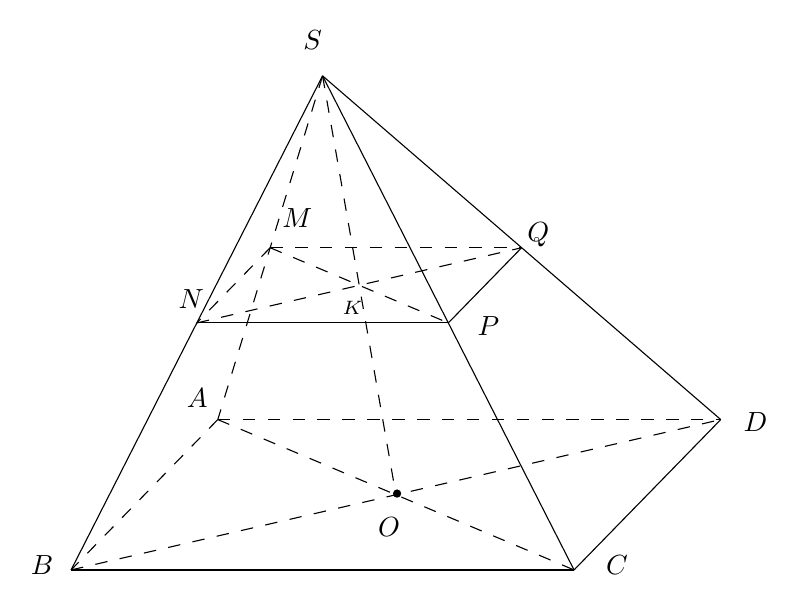
\begin{tikzpicture}[x=0.75pt,y=0.75pt,yscale=-1,xscale=1]
					\draw [dash pattern={on 4.5pt off 4.5pt}] (163.12,202.05) --  (405.44,202.05);
					 \draw (92.44,274.5) -- (334.76,274.5);
					\draw [dash pattern={on 4.5pt  off 4.5pt}] (163.12,202.05) -- (92.44,274.5);
					 \draw (405.44,202.05) -- (334.76,274.5);
					\draw [dash pattern={on 4.5pt off 4.5pt}] (213.6,36.45)  -- (163.12,202.05);
					\draw (213.6,36.45) -- (92.44,274.5); 
					\draw  (213.6,36.45) -- (405.44,202.05);
					\draw (213.6,36.45) -- (334.76,274.5); 
					\draw [dash pattern={on 4.5pt off 4.5pt}] (163.12,202.05) -- (334.76,274.5); 
					\draw [dash pattern={on 4.5pt off 4.5pt}]  (92.44,274.5) -- (405.44,202.05);
					\draw [dash pattern={on 4.5pt off 4.5pt}]  (213.6,36.45) -- (248.94,238.27);
					\draw [line width=3] [line join = round][line cap = round] (249.5,237.7).. controls (249.5,237.7) and (249.5,237.7)..  (249.5,237.7);
					\draw [dash pattern={on 4.5pt off 4.5pt}] (188.36,119.25) --  (309.52,119.25);
					\draw (153.02,155.48) --  (274.18,155.48);
					\draw [dash  pattern={on 4.5pt off 4.5pt}] (188.36,119.25) -- (153.02,155.48);
					\draw (309.52,119.25) -- (274.18,155.48); 
					\draw [dash pattern={on 4.5pt off 4.5pt}] (188.36,119.25) -- (274.18,155.48); 
					\draw [dash pattern={on 4.5pt off 4.5pt}] (153.02,155.48) -- (309.52,119.25); 
					\draw  (203.05,13.5) node [anchor=north west][inner sep=0.75pt] [align=left] {$S$};
					\draw (146.96,186)  node [anchor=north west][inner sep=0.75pt] [align=left] {$A$};
					 \draw (71.79,266.5) node [anchor=north west][inner sep=0.75pt] [align=left] {$B$};
					 \draw (348.96,266.5) node [anchor=north west][inner sep=0.75pt] [align=left] {$C$};
					\draw  (415.15,197.5) node [anchor=north west][inner sep=0.75pt] [align=left] {$D$};
					\draw (239.07,248.1)  node [anchor=north west][inner sep=0.75pt] [align=left] {$O$};
					\draw  (222,144) node [anchor=north west][inner sep=0.75pt] [font=\scriptsize] [align=left] {\textbf{$K$}};
					\draw (193,99) node [anchor=north west][inner sep=0.75pt]  [align=left] {$M$};
					\draw (143,138) node [anchor=north  west][inner sep=0.75pt] [align=left] {$N$};
					\draw  (311,106) node [anchor=north west][inner sep=0.75pt] [align=left] {$Q$};
					\draw (287,151)  node [anchor=north west][inner sep=0.75pt] [align=left] {$P$};
				\end{tikzpicture}
		\end{center}
		 Gọi $ O=AC\cap BD$ và $ K=SO\cap MP$. Khi đó $NK$ cắt $SD$. Gọi $ Q=NK\cap SD$.\\
	Ta có  $ (MNPQ)\equiv (MNP)\Rightarrow $ Thiết diện của hình chóp $S.ABCD$ cắt bởi mặt phẳng $(MNP)$ là tứ giác $MNPQ$.}
\end{ex}

% nguồn: Ok_TracNghiemLop11_Lan1
\begin{ex}%[1H4V2-5]%[ma:14c0b877]
	Cho tứ diện $ABCD$ có $M$ và $N$ theo thứ tự là trung điểm của $AB$ và $AC$. Mặt phẳng $\left(\alpha\right)$ qua $MN$ cắt tứ diện $ABCD$ theo thiết diện là đa giác $(T)$. Khẳng định nào sau đây đúng? 
	\choice 
		{$(T)$ là hình bình  hành}
		{$(T)$ là tam giác} 
		 {\True $(T)$ là tam giác hoặc hình thang}
		 {$(T)$ là hình thoi}
	\loigiai{ 
		\begin{center}
			\begin{tikzpicture}[line join=round,line cap=round,>=stealth,scale=0.65,font=\footnotesize]
					\foreach \x/\y/\n in {0/0/B,2.5/-2/C,6/0/D} \coordinate (\n) at  (\x,\y);
					\coordinate (A)  at ($(B)+(2,4)$);
					\coordinate (M) at  ($(A)!1/2!(B)$);
					\coordinate (N) at  ($(A)!1/2!(C)$);
					\coordinate (P) at ($(C)!1/3!(D)$); 
					\coordinate (Q) at ($(B)!1/3!(D)$); 
					\coordinate (K) at ($(A)!3/4!(D)$); 
					\draw (A)--(B)--(C)--(D)--(A)--(C) 
						(M)--(N)--(P) 
						 (N)--(K);
					\draw[dashed] (B)--(D) 
						(M)--(Q)--(P) 
						(K)--(M); 
					\foreach \t/\g  in {A/90,B/180,C/-90,D/0,P/-90,Q/-135,M/180,N/45,K/20}{
						 \draw[fill] (\t) circle (1pt) node[shift={(\g:8pt)}]{$ \t $};
					 }
				\end{tikzpicture}
		\end{center}
		Ta có các trường  hợp sau:
		\begin{itemize}
			\item $\left(\alpha\right)$ giao với cạnh $AD$ của tứ  diện $ABCD$ tại $K$. \\
			 Khi đó dễ thấy thiết diện $(T)$ là tam giác $MNK$. \\
			Đặc biệt, nếu $K\equiv D$ thì thiết diện $(T)$ là tam giác $MND$; nếu $K\equiv A$ thì  thiết diện $(T)$ là tam giác $ABC$.
			\item  $\left(\alpha\right)$ giao với cạnh $CD$ của tứ diện $ABCD$ tại $P$ ($P\not\equiv D$, $P\not\equiv C$).\\
			Khi đó, $P$ là một điểm chung của $\left(\alpha\right)$ và $\left(BCD\right)$. Hơn nữa, ta có $MN\parallel BC$ (tính chất đường trung bình của  tam giác), $BC\subset\left(BCD\right)$ nên suy ra $MN\parallel \left(BCD\right)$. \\
			Do đó $\left(\alpha\right)\cap\left(BCD\right)=PQ$ với $PQ\parallel MN$ và $Q\in  BD$. \\
			Từ đó, dễ thấy thiết diện $(T)$ là  hình thang $MNPQ$.\\
			Đặc biệt, khi $P$ là trung điểm của $CD$ thì $Q$ cũng là trung điểm của $BD$. Do đó $NP\parallel AD\parallel MQ$ (tính chất đường trung bình của tam giác). Suy ra thiết  diện $MNPQ$ là hình bình hành.\\
			Ngoài ra, nếu $P\equiv D$ thì thiết diện $(T)$ là tam giác $MND$. Nếu $P\equiv  C$ thì $Q\equiv B$ và thiết diện $(T)$ là tam giác $ABC$.
		\end{itemize}
		Vậy, thiết diện $(T)$ của tứ diện $ABCD$ khi cắt bởi $\left(\alpha\right)$ là  một tam giác hoặc một hình thang (chú ý hình bình hành cũng là hình thang).
	 }
\end{ex}

% nguồn: Ok_TracNghiemLop11_Lan1
\begin{ex}%[1H4V2-5]%[ma:f89a295a]
	Cho tứ diện $ABCD$. Gọi $N$ và $P$ lần lượt là trung điểm  của các cạnh $BD$ và $AD$; $M$ là điểm thuộc đoạn $BC$ sao cho $MC=2MB$. Kết luận nào sau đây đúng nhất về thiết diện của mặt phẳng $\left(MNP\right)$ với hình chóp $ABCD$?
	\choice 
		{Thiết diện là ngũ  giác}
		 {Thiết diện là hình bình hành}
		{\True Thiết diện là hình  thang}
		{Thiết diện  là tứ giác}
	\loigiai{ 
	\immini{ 
		 Ta có $NP$ là đường trung bình của $\triangle DAB$ nên $NP\parallel AB$.\\
		Khi  đó $\heva{&M\in \left(MNP\right)\cap\left(ABC\right)\\
		&NP\parallel AB\\ 
		 &NP\subset\left(MNP\right),AB\subset\left(ABC\right)}\Rightarrow Mx\parallel AB$.\\
		Gọi $Q=Mx\cap  AC$.\\
		Suy ra $\left(MNP\right)\cap\left(ABC\right)=MQ$ và $\left(MNP\right)\cap\left(ACD\right)=QP$.\\ 
		Do đó thiết diện của mặt phẳng $\left(MNP\right)$ với hình chóp $ABCD$ là hình thang $MNPQ$  (vì $PN\parallel MQ\parallel AB$).
		}{\begin{tikzpicture}[line join=round,line cap=round,>=stealth,scale=0.6,font=\footnotesize]
		\foreach \x/\y/\n in {0/0/B,1.5/-2/C,6/0/D} \coordinate (\n)  at (\x,\y);
		 \coordinate (A) at ($(B)+(2,4)$);
		 \coordinate (N) at ($(B)!1/2!(D)$);
		\coordinate (M) at ($(B)!1/3!(C)$); 
		 \coordinate (P) at ($(A)!1/2!(D)$);
		 \coordinate (Q) at ($(A)!1/3!(C)$);
		\draw (A)--(B)--(C)--(D)--(A)--(C) 
			(M)--(Q)--(P); 
		\draw[dashed]  (B)--(D)
			 (M)--(N)--(P)--(M);
		\foreach \t/\g in {A/90,B/180,C/-90,D/0,P/45,Q/130,M/200,N/-90}{ 
			\draw[fill] (\t) circle (1pt) node[shift={(\g:8pt)}]{$ \t $}; 
		 }
	\end{tikzpicture}
		 }
	} 
\end{ex}

% nguồn: Ok_TracNghiemLop11_Lan1
\begin{ex}%[1H4V2-5]%[ma:750a073e]
	Cho hình chóp $S.ABCD$ có đáy $ABCD$ là hình bình hành tâm $O$. Gọi $I$ là điểm trên cạnh  $SO$. Mặt phẳng $\left(ICD\right)$ cắt hình chóp theo thiết diện là hình gì?
	 \choice
		{Tam  giác}
		 {\True Hình thang}
		{Hình  bình hành}
		{Hình  chữ nhật}
	\loigiai{ 
		\begin{center}
			\begin{tikzpicture}[line join=round,line cap=round,>=stealth,scale=0.85,font=\footnotesize]
					\foreach \x/\y/\n in  {0/0/A,-2.5/-2/B,6/0/D} \coordinate (\n) at (\x,\y);
					\coordinate  (C) at ($(B)+(D)-(A)$);
					\coordinate (S) at  ($(A)+(1,4)$);
					\coordinate (O) at ($(B)!0.5!(D)$); 
					\coordinate (E) at  ($(S)!0.4!(A)$);
					\coordinate (F)  at ($(S)!0.4!(B)$);
					\path 
						(intersection of C--E  and S--O) coordinate (I);
					\draw  (S)--(B)--(C)--(D)--(S)--(C)--(F);
					\draw[dashed]  (S)--(A)--(D)--(B)
						 (C)--(A)--(B)
						(E)--(C) 
						(S)--(O) 
						(F) 
						 (I)--(D)--(E)--(F);
					\foreach \t/\g in {A/150,B/-150,C/-30,D/30,S/90,O/-90,E/30,F/170,I/40}{ 
						\draw[fill] (\t) circle  (1pt) node[shift={(\g:7pt)}]{$ \t $};
					 }
				\end{tikzpicture}
		\end{center}
		Ta  có $\heva{&\left(ICD\right)\cap\left(SCD\right)=CD\\&
		\left(ICD\right)\cap\left(ABCD\right)=CD.}$ \quad$(1)$\\ 
		Trong  $\left(SAC\right)$, gọi $E=IC\cap SA\Rightarrow\left(ICD\right)\equiv\left(ECD\right)$ $\Rightarrow\left(ECD\right)\cap\left(SAD\right)=ED$,\quad $(2)$\\
		Vì $AB\parallel CD$ nên $\left(ECD\right)\cap\left(SAB\right)$ theo giao  tuyến là đường thẳng đi qua $E$ và song song với $AB$, $CD$ cắt $SB$ tại $F$ $\Rightarrow\left(ECD\right)\cap\left(SAB\right)=EF$.\quad $(3)$\\
		Từ $(1)$, $(2)$ và $(3)$ suy ra $\left(ICD\right)$ cắt hình chóp theo thiết diện  là tứ giác $CDEF$.\\
	 Vì $EF\parallel AB\parallel CD$ nên tứ giác $CDEF$ là hình thang.}
\end{ex}

% nguồn: Ok_Toan11_TracNghiem_Lan2
\begin{ex}%[1H4C2-5]%[ma:5d1a1ca5]
	Cho hình chóp $S.ABCD$ có đáy $ABCD$ là hình thang $\left(AB \parallel  CD\right)$, cạnh $AB=3a$, \break $AD=CD=a$. Tam giác $SAB$ cân tại $S$, $SA=2a$. Mặt phẳng $(P)$ song song với $SA$, $AB$ cắt các cạnh $AD$, $BC$, $SD$, $SB$ theo thứ tự tại $M$, $N$, $P$, $Q$. Đặt $AM=x$, ($0<x<a$). Biết $x$ là giá trị để tứ giác $MNPQ$ ngoại tiếp được một đường tròn, bán kính đường tròn đó bằng
	\choice 
		 {\True $\dfrac{a\sqrt{7}}{6}$}
		 {$\dfrac{a\sqrt{7}}{4}$}
		{$\dfrac{3a}{4}$} 
		 {$a$}
	\loigiai{ 
		\begin{center}
			\begin{tikzpicture}[scale=1,font=\footnotesize,line join=round,line cap=round,>=stealth]
					 \coordinate[label=left:$A$] (A) at (0,0);
					\coordinate[label=below left:$D$] (D)  at (-50:2);
					 \coordinate[label=below right:$C$] (C) at (-30:3);
					\coordinate[label=right:$B$]  (B) at (4,0);
					\coordinate[label=above:$S$] (S) at  (65:4);
					\coordinate[label=left:$E$] (E)  at ($(S)!0.2!(A)$);
					 \coordinate[label=left:$M$] (M) at ($(A)!0.5!(D)$);
					\coordinate[label=right:$N$] (N)  at ($(B)!0.5!(C)$);
					\coordinate[label=right:$F$] (F) at  ($(S)!0.2!(B)$);
					\coordinate[label=left:$Q$] (Q)  at ($(S)!0.5!(D)$);
					\coordinate[label=right:$P$] (P)  at ($(S)!0.5!(C)$);
					\coordinate[label=below:$I$] (I) at (intersection of A--D  and B--C);
					\draw  (A)--(D)--(C)--(B)--(S)--cycle (D)--(S)--(C)
						(M)--(Q)--(P)--(N) 
						(D)--(I)--(C); 
					\draw[dashed] (A)--(B) 
						(E)--(F) 
						(M)--(N); 
					\foreach \diem in {A,D,C,B,S,E,F,M,N,P,Q,I} \fill (\diem) circle  (1pt);
				\end{tikzpicture}
		\end{center}
		Ta có $(P)$ song song với $SA$, $AB$ cắt các cạnh $AD$, $BC$, $SD$, $SB$ tại $M$,  $N$, $P$, $Q$ theo thứ tự tại $M$, $N$, $P$, $Q$.\\
		Suy ra  $\heva{
		&MN\parallel AB\parallel PQ\\ &MQ\parallel  SA\\ &NP\parallel SB.
		 }$\\
		Theo công thức Hê-rông, diện  tích tam giác $SAB$ là
		 $S_{SAB}=\dfrac{3\sqrt{7}}{4}a^2$.\\
		Gọi  $r_1$ là bán kính đường tròn nội tiếp tam giác $SAB$. Suy ra
		$r_1=\dfrac{S}{p}=\dfrac{3\sqrt{7}}{14}a$.\\ 
		Gọi $E$, $F$ nằm trên cạnh $SA$, $SB$ sao cho $EF\parallel AB$ và tiếp xúc với đường tròn  nội tiếp $\triangle ABC$.\\
		 Khi đó khoảng cách $AB$ và $EF$ là $d=2r_1=\dfrac{3\sqrt{7}}{7}a$.\\
		Gọi $h$ là dường cao của tam giác $SAB$,  ta có
		\[h=\sqrt{SA^2-\dfrac{AB^2}{4}}=\dfrac{\sqrt{7}}{2}a. \] 
		Suy  ra
		\[\dfrac{SE}{SA}=\dfrac{h-d}{h}=\dfrac{1}{7}.\] 
		Ta  có
		\[\dfrac{AM}{AD}=\dfrac{SQ}{SD}=\dfrac{QP}{DC}\Rightarrow  QP=AM=x.\]
		Mặt khác,  gọi $I$ là giao điểm của $AD$ và $BC$, khi đó, ta được
		\[\dfrac{MN}{AB}=\dfrac{IM}{IA}=\dfrac{3a-2x}{3a}\Rightarrow  MN=3a-2x.\]
		Điều kiện để hình thang $MNPQ$ ngoại tiếp đường tròn là hai hình thang $MNPQ$ và $ABEF$  đồng dạng với nhau. Khi đó, ta được
		 \[\dfrac{QP}{MN}=\dfrac{EF}{AB}=\dfrac{1}{7}\Rightarrow\dfrac{x}{3a-2x}=\dfrac{1}{7}\Rightarrow x=\dfrac{a}{3}.\]
		Gọi $r_2$ là bán kính  đường tròn nội tiếp hình thang $MNPQ$.\\
		 Ta có
		\[\dfrac{r_2}{r_1}=\dfrac{MN}{AB}=\dfrac{3a-2x}{3a}=\dfrac{7}{9}\Rightarrow  r_2=\dfrac{a\sqrt{7}}{6}.\]
	} 
\end{ex}


%%%%%%%%%%%%%%%% TRẢ LỜI NGẮN %%%%%%%%%%%%%%%%

% nguồn: Ok_TraLoiNgan_Lop11_Lan1
\begin{ex}%[1H4V2-5]%[ma:c9c0fca7]
	Cho hình chóp $S.ABCD$ có đáy $ABCD$ là hình bình hành tâm $O$. Gọi $M$, $I$, $J$ lần lượt là trung điểm của  $OB$, $AB$ và $SA$. Thiết diện của hình chóp $S.ABCD$ khi cắt bởi mặt phẳng $(MIJ)$ là một đa giác có số cạnh là bao nhiêu?
	 \shortans{5}
	 \loigiai{
		\begin{center}
			\begin{tikzpicture}[line join=round,line cap=round,>=stealth,scale=0.75,font=\footnotesize]
					\foreach \x/\y/\n in {0/0/A,-2.5/-2/B,6/0/D} \coordinate  (\n) at (\x,\y);
					\coordinate (C) at  ($(B)+(D)-(A)$);
					 \coordinate (S) at ($(A)+(1.5,4)$);
					 \coordinate (O) at ($(B)!1/2!(D)$);
					\coordinate (M) at  ($(B)!1/2!(O)$);
					\coordinate (I) at  ($(B)!1/2!(A)$);
					\coordinate (J) at  ($(S)!1/2!(A)$);
					\coordinate (H)  at ($(B)!1/2!(C)$);
					\coordinate (L) at  ($(S)!1/2!(C)$);
					\coordinate (K) at  ($(S)!1/4!(D)$);
					\draw (S)--(B)--(C)--(D)--(S)--(C) 
						 (H)--(L)--(K);
					\draw[dashed] (S)--(A)--(D) 
						(C)--(A)--(B)--(D) 
						 (J)--(K)--(M)--(J)--(I)--(H);
					\foreach \t/\g in  {A/150,B/-150,C/-30,D/30,S/90,O/-90,M/-90,J/150,I/170,H/-90,L/20,K/60}{
						\draw[fill=black] (\t) circle (1pt) node[shift={(\g:7pt)}]{$  \t $};
					 }
				\end{tikzpicture}
		\end{center}
		\begin{itemize}
			\item  Trong $(ABCD)$, gọi $H=IM\cap BC$.
			\item $\heva{&H\in (MIJ)\cap (SBC)\\&IJ\parallel SB}\Rightarrow (MIJ)\cap (SBD)=HL$ với $L\in SC$ và $HL\parallel  SB$.
			\item $\heva{&M\in (MIJ)\cap (SBD)\\&IJ\parallel SB}\Rightarrow (MIJ)\cap (SBD)=MK$ với $K\in  SD$ và $MK\parallel SB$.
			\item Suy ra $\heva{&(MIJ)\cap  (ABCD)=HI\\&(MIJ)\cap(SAB)=IJ\\&(MIJ)\cap(SAC)=JK\\&(MIJ)\cap(SCD)=KL\\&(MIJ)\cap(SBC)=LH}\Rightarrow$ thiết diện là ngũ giác $HIJKL$.
		\end{itemize}
	} 
\end{ex}

% nguồn: Ok_TraLoiNgan_Lop11_Lan2
\begin{ex}%[1H4V2-5]%[ma:509015e1]
	Cho hình chóp $S.ABCD$ có đáy là hình thang và $AD\parallel BC$, $AB=2$, $AD=8$, $BC=4$, $\widehat{BAD}=60^\circ$. Mặt phẳng $(\alpha)$ song song với $(ABCD)$ và cắt cạnh $SA$ tại $M$ sao cho  $\dfrac{SA}{SM}=3$. Tính diện tích của thiết diện tạo bởi $(\alpha)$ và hình chóp $S.ABCD$ (làm tròn kết quả đến hàng phần trăm).
	\shortans{1,15} 
	 \loigiai{
		\begin{center}
			\begin{tikzpicture}[scale=1,font=\footnotesize,line join=round,line cap=round,>=stealth]
					\coordinate[label=left:$A$] (A)  at (0,0);
					\coordinate[label=below left:$B$] (B) at (-55:2); 
					 \coordinate[label=below right:$C$] (C) at (-30:3.2);
					\coordinate[label=right:$D$] (D) at  (4,0);
					\coordinate[label=above:$S$] (S) at  (65:4);
					\coordinate[label=left:$M$] (M) at ($(S)!1/3!(A)$); 
					\coordinate[label=left:$N$] (N) at ($(S)!1/3!(B)$); 
					\coordinate[label=right:$P$] (P)  at ($(S)!1/3!(C)$);
					\coordinate[label=right:$Q$] (Q) at  ($(S)!1/3!(D)$);
					 \coordinate[label=above left:$H$] (H) at ($(A)!(B)!(D)$);
					\path[pattern = north east  lines] (M)--(N)--(P)--(Q)--cycle;
					\draw (A)--(B)--(C)--(D)--(S)--cycle (B)--(S)--(C) 
						(M)--(N)--(P)--(Q); 
					 \draw[dashed] (A)--(D)
						 (M)--(Q)
						(B)--(H); 
					\foreach \diem in {A,B,C,D,S,M,N,P,Q,H} \fill  (\diem) circle (1pt);
				\end{tikzpicture}
		\end{center}
		Gọi $H$ là hình chiếu của $B$ lên cạnh  $AD$.\\
		 Suy ra $BH=AB\cdot\sin 60^{\circ}=\sqrt{3}$.\\
		Ta  có
		$S_{ABCD}=\dfrac{(AB+BC)\cdot BH}{2}=\dfrac{(8+4)\cdot\sqrt{3}}{2}=6\sqrt{3}$.\\ 
		Gọi  $N$, $P$, $Q$ lần lượt là giao điểm của $(\alpha)$ với các cạnh $SB$, $SC$, $SD$.\\
		Vì $(\alpha)\parallel(ABCD)$ nên  thiết diện $MNPQ$ là hình thang.\\ Ta lại có $\dfrac{SA}{SM}=3$. Suy ra $\dfrac{SM}{SA}=\dfrac{1}{3}$.\\ Theo định lý Talet, ta có
		 \[\dfrac{MN}{AB}=\dfrac{NP}{BC}=\dfrac{PQ}{CD}=\dfrac{QM}{AD}=k=\dfrac{1}{3}.\]
		Diện tích thiết diện $MNPQ$  bằng
		\[S_{MNPQ}=k^2\cdot S_{ABCD}=\dfrac{1}{9}\cdot 6\sqrt{3}=\dfrac{2\sqrt{3}}{3}\approx  1{,}15.\]
	} 
\end{ex}

% nguồn: Ok_TraLoiNgan_Lop11_Lan2
\begin{ex}%[1H4V2-5]%[ma:0bb1647b]
	Cho tứ diện đều $ABCD$ cạnh bằng $a$. Gọi $M$, $N$, $P$ tương ứng là trung điểm của $AB$, $BC$, $CD$. Mặt phẳng $(MNP)$ tạo với hình tứ diện một  thiết diện có diện tích là $S$. Khi $a=2$ thì giá trị của $S$ bằng bao nhiêu?
	 \shortans{1}
	 \loigiai{
		\begin{center}
			\begin{tikzpicture}[scale=0.7,font=\footnotesize,line join=round,line cap=round,>=stealth]
					 \path
						(0,0)  coordinate (B)
						++ (0:6)  coordinate (D)
						++ (-150:4) coordinate  (C)
						(4,5) coordinate (A) 
						($(A)!1/2!(B)$)  coordinate (M)
						 ($(B)!1/2!(C)$) coordinate (N)
						($(C)!1/2!(D)$)  coordinate (P)
						($(A)!1/2!(D)$) coordinate (Q); 
					\draw  (A)--(B)--(C)--(D)--(A)--(C)
						 (M)--(N)
						 (P)--(Q);
					\draw[dashed]  (P)--(B)--(D)
						(N)--(P)--(M)--(Q)--(N); 
					\foreach \i/\j  in {A/90,B/180,C/0,D/-90,M/180,N/-90,P/-90,Q/30}{
						\draw (\i) circle (1pt)  node[shift={(\j:3mm)}] {$\i$};
					} 
				\end{tikzpicture}
		\end{center}
		Do $M$, $N$, $P$ tương ứng là trung điểm của $AB$, $BC$, $CD$ suy ra  $MN \parallel AC$, $NP\parallel BD$ nên mặt phẳng $(MNP)$ cắt $AD$ tại $Q$ và có $MQ\parallel BD$, $PQ\parallel AC$.\\
		Ta có $MN=PQ=\dfrac{1}{2}AC=\dfrac{a}{2}$; $MQ=NP=\dfrac{1}{2}BD=\dfrac{a}{2}\Rightarrow MNPQ$ là  hình thoi.\\
		Vì các tam  giác $BCD$, $ACD$ đều cạnh $a$ nên đường cao $BP=AP=\dfrac{a\sqrt{3}}{2}$.\\
		Khi đó tam giác $ABP$ cân  tại $P$ nên đường cao $MP=\sqrt{BP^2-BM^2}=\dfrac{a\sqrt{2}}{2}$.\\
		Tương tự ta  tính được $NQ=\dfrac{a\sqrt{2}}{2}$.\\
		Do đó diện tích thiết  diện là $S=\dfrac{1}{2}MP\cdot NQ=\dfrac{a^2}{4} \xrightarrow{a=2} S=1$.
	 }
\end{ex}

% nguồn: Ok_TraLoiNgan_Lop11_Lan2
\begin{ex}%[1H4V2-5]%[ma:aa3ed624]
	Cho hình chóp tứ giác đều $S.ABCD$ có cạnh đáy bằng $10$. Gọi $M$ là điểm trên $SA$ sao cho $\dfrac{SM}{SA}=\dfrac{2}{3}$. Một mặt phẳng $(\alpha)$ đi qua $M$ song  song với $AB$ và $BC$, cắt hình chóp theo một tứ giác, tính diện tích của tứ giác đó (làm tròn kết quả đến hàng phần mười).
	\shortans{44,4} 
	\loigiai{ 
		\begin{center}
			\begin{tikzpicture}[scale=1,font=\footnotesize,line join=round,line cap=round,>=stealth]
					\coordinate[label=below left:$A$] (A) at  (0,0);
					\coordinate[label=below:$D$]  (D) at (-20:3);
					\coordinate[label=above right:$B$] (B) at (4,0); 
					\coordinate[label=right:$C$] (C)  at ($(B)-(A)+(D)$);
					\coordinate[label=below:$O$] (O) at  ($(A)!.5!(C)$);
					\coordinate[label=above:$S$]  (S) at ($(O)+(90:4)$);
					\coordinate[label=left:$M$] (M) at  ($(S)!2/3!(A)$);
					 \coordinate[label=above right:$N$] (N) at ($(S)!2/3!(B)$);
					 \coordinate[label=right:$P$] (P) at ($(S)!2/3!(C)$);
					\coordinate[label=below left:$Q$] (Q) at ($(S)!2/3!(D)$); 
					 \path[pattern = north east lines] (M)--(N)--(P)--(Q)--cycle;
					\draw  (A)--(D)--(C)--(S)--cycle (S)--(D)
						 (M)--(Q)--(P);
					\draw[dashed] (D)--(B)--(A)--(O) 
						(S)--(O)--(C)--(B)--cycle (M)--(N)--(P); 
					\foreach \diem in  {A,D,C,B,O,S,M,N,P,Q} \fill (\diem) circle (1pt);
				\end{tikzpicture}
		\end{center}
		Mặt phẳng $(\alpha)$ đi qua $M$ và song song với $AB$ nên từ $M$ kẻ  đường thẳng song song với $AB$ cắt $SB$ tại $N$, từ $N$ kẻ đường thẳng song song với $BC$ cắt $SC$ tại $P$.\\
		Từ $P$ kẻ đường thẳng song song  với $CD$ cắt $SD$ tại $Q$.\\
		Khi  đó mặt phẳng $(\alpha)$ cắt hình chóp theo tứ giác $MNPQ$.\\
		Ta có tứ giác $MNPQ$  là hình vuông có cạnh $MN=\dfrac{2}{3}AB=\dfrac{20}{3}$.\\
		Vậy  diện tích tứ giác $MNPQ$ bằng
		\[S=\left(\dfrac{20}{3}\right)^2=\dfrac{400}{9}\approx 44{,}4.\] 
	} 
\end{ex}

% nguồn: Ok_TraLoiNgan_Lop11_Lan2
\begin{ex}%[1H4V2-5]%[ma:1b2ede1b]
	Cho hai hình vuông $ABCD$ và $CDIS$ không thuộc một mặt phẳng và  cạnh bằng $4$. Biết tam giác $SAC$ cân tại $S$, $SB=8$. Gọi $S$ là diện tích thiết diện của mặt phẳng $(ACI)$ và hình chóp $S.ABCD$. Tính $\dfrac{S}{\sqrt{2}}$.
	\shortans{8} 
	 \loigiai{
		\begin{center}
			\begin{tikzpicture}[scale=1,font=\footnotesize,line join=round,line cap=round,>=stealth]
					\coordinate[label=below left:$C$] (C) at (0,0); 
					\coordinate[label=below:$B$] (B) at  (-50:3);
					\coordinate[label=below:$D$] (D) at  (4,0);
					\coordinate[label=right:$A$] (A) at ($(D)-(C)+(B)$); 
					 \coordinate[label=below:$N$] (N) at ($(C)!.5!(A)$);
					\coordinate[label=above:$S$] (S) at  ($(N)+(70:4)$);
					\coordinate[label=above right:$O$] (O)  at ($(S)!0.5!(D)$);
					\coordinate[label=right:$I$] (I) at  ($(S)-(C)+(D)$);
					\path[pattern =  north east lines] (C)--(O)--(A);
					 \draw (C)--(B)--(A)--(S)--cycle (A)--(I)--(S)--(B);
					 \draw[dashed] (B)--(D)--(C)--(N)
						(S)--(A)--(D)--cycle  (C)--(O)--(A)--(N)--(O)--(I)--(B)
						 (I)--(D);
					\draw (D)  node[below]{$D$};
					\foreach  \diem in {C,B,A,D,N,S,O,I} \fill (\diem) circle (1pt);
				\end{tikzpicture}
		\end{center}
		Gọi $O=SD\cap  CI$, $N=AC\cap BD$.\\
		Suy ra  $O$, $N$ lần lượt là trung điểm của $DS$, $DB$.\\
		Khi  đó $ON=\dfrac{1}{2}\cdot SB=4$.\\
		Thiết diện của mặt phẳng $(ACI)$  và hình chóp $S.ABCD$ là tam giác $OCA$.\\
		Ta có tam giác $\triangle SAC$ cân  tại $S$.\\
		Suy ra $SC=SA\Rightarrow  \triangle SDC=\triangle SDA$.\\
		Khi đó, ta được $CO=AO$  (cùng là đường trung tuyến của hai đỉnh tương ứng).\\
		 Suy ra $\triangle OCA$ cân tại $O$.\\
		 Vậy
		\[S_{\triangle  OCA}=\dfrac{1}{2}ON\cdot AC=\dfrac{1}{2}\cdot4\cdot4\sqrt{2}=8\sqrt{2}\Rightarrow \dfrac{S}{\sqrt{2}}=8.\]
	 }
\end{ex}

% nguồn: Ok_TraLoiNgan_Lop11_Lan2
\begin{ex}%[1H4V2-5]%[ma:e1e97ea2]
	Cho hình chóp $S.ABCD$ có đáy $ABCD$ là hình thang với  các cạnh đáy là $AB$ và $CD$. Gọi $I$, $J$ lần lượt là trung điểm của các cạnh $AD$ và $BC$, $G$ là trọng tâm của tam giác $SAB$. Biết tứ giác tạo bởi các giao tuyến của mặt phẳng $(IJG)$ và các mặt của hình chóp là một hình bình hành, $AB=6$. Khi đó, độ dài cạnh $CD$ bằng bao nhiêu?
	 \shortans{2}
	 \loigiai{
		\begin{center}
			\begin{tikzpicture}[scale=1,font=\footnotesize,line join=round,line cap=round,>=stealth]
					 \coordinate[label=left:$A$] (A) at (0,0);
					\coordinate[label=below  left:$D$] (D) at (-50:2);
					\coordinate[label=below right:$C$] (C) at  (-30:3);
					\coordinate[label=right:$B$] (B)  at (4,0);
					\coordinate[label=above:$S$] (S) at  (65:4);
					\coordinate[label=left:$E$]  (E) at ($(A)!0.5!(D)$);
					\coordinate[label=below:$I$] (I) at ($(A)!0.5!(B)$); 
					\coordinate[label=right:$J$] (J) at ($(B)!0.5!(C)$); 
					\coordinate[label=left:$F$] (F)  at ($(S)!2/3!(A)$);
					 \coordinate[label=right:$H$] (H) at ($(S)!2/3!(B)$);
					\coordinate[label=above left:$G$]  (G) at (intersection of F--H and S--I);
					\draw  (A)--(D)--(C)--(B)--(S)--cycle (D)--(S)--(C)
						 (E)--(F)
						(H)--(J); 
					\draw[dashed] (A)--(B) 
						(E)--(G)--(J)--cycle (F)--(H) 
						(S)--(I); 
					\foreach  \diem in {A,D,C,B,S,E,F,I,J,H,G} \fill (\diem) circle (1pt);
				\end{tikzpicture}
		\end{center}
		Kẻ đường thẳng qua $G$ song song với  $AB$ cắt $SA$ tại $F$, cắt $SB$ tại $H$.\\
		Khi đó, tứ giác $IJHF$  là tứ giác tạo bởi các giao tuyến của $(IJG)$ và các mặt của hình chóp.\\
		Suy ra  tứ giác $IJHF$ là hình bình hành.\\
		Gọi $E$ là trung điểm $AB$. Ta  có $\dfrac{SG}{SE}=\dfrac{2}{3}$.\\
		Vì $I$, $J$ lần lượt là trung điểm của $AD$ và $BC$ nên $IJ$ là đường trung bình của hình thang  $ABCD$.\\
		Suy ra $FH\parallel  IJ\parallel AB$.\\
		Ta  có
		\[\dfrac{FH}{AB}=\dfrac{SG}{SE}=\dfrac{2}{3}\Rightarrow  FH=\dfrac{2}{3}\cdot AB=\dfrac{2}{3}\cdot6=4\Rightarrow IJ=4.\]
		Do $IJ=\dfrac{AB+CD}{2}$.\\ 
		Suy ra  $CD=2IJ-AB=2\cdot4-6=2$.
	 }
\end{ex}

% nguồn: Ok_TraLoiNgan_Lop11_Lan2
\begin{ex}%[1H4V2-5]%[ma:f78ced67]
	Cho hình chóp tứ giác đều $S.ABCD$ có cạnh đáy bằng $10$. Gọi $M$ là điểm nằm trên cạnh $SA$ sao cho $\dfrac{SM}{SA}=\dfrac{2}{3}$. Mặt phẳng $(P)$ qua $M$ và song song với $AB$ và $AD$. Xác định thiết diện của $(P)$ với hình chóp $S.ABCD$. Tính  diện tích thiết diện này (kết quả làm tròn đến hàng phần chục).
	 \shortans{44,4}
	 \loigiai{
		\begin{center}
			\begin{tikzpicture}[scale=1,font=\footnotesize,line join=round,line cap=round,>=stealth]
					\coordinate[label=below left:$A$]  (A) at (0,0);
					\coordinate[label=below:$D$] (D)  at (-20:3);
					\coordinate[label=above right:$B$] (B)  at (4,0);
					\coordinate[label=right:$C$] (C) at ($(B)-(A)+(D)$); 
					\coordinate[label=below:$O$]  (O) at ($(A)!.5!(C)$);
					\coordinate[label=above:$S$] (S)  at ($(O)+(90:4)$);
					 \coordinate[label=left:$M$] (M) at ($(S)!2/3!(A)$);
					 \coordinate[label=above right:$N$] (N) at ($(S)!2/3!(B)$);
					\coordinate[label=right:$P$] (P) at  ($(S)!2/3!(C)$);
					\coordinate[label=below left:$Q$] (Q)  at ($(S)!2/3!(D)$);
					\path[pattern = north east lines]  (M)--(N)--(P)--(Q)--cycle;
					 \draw (A)--(D)--(C)--(S)--cycle (S)--(D)
						 (M)--(Q)--(P);
					\draw[dashed]  (D)--(B)--(A)--(O)
						(S)--(O)--(C)--(B)--cycle (M)--(N)--(P); 
					\foreach \diem in {A,D,C,B,O,S,M,N,P,Q} \fill  (\diem) circle (1pt);
				\end{tikzpicture}
		\end{center}
		Mặt phẳng $(SAB)$ chứa đường thẳng $AB$ song song với mặt phẳng $(P)$  nên mặt phẳng $(SAB)$ cắt mặt phẳng $(P)$ theo giao tuyến song song với $AB$.\\
		Qua $M$ kẻ $MN\parallel AB$  $(N\in SB)$ thì $MN$ là giao tuyến của mặt phẳng $(P)$ và mặt phẳng $(SAB)$.\\
		Mặt phẳng $(SAD)$ chứa đường thẳng $AD$ và song song  với mặt phẳng $(P)$ nên mặt phẳng $(SAD)$ cắt mặt phẳng $(P)$ theo giao tuyến song song với $AD$.\\
		Qua $M$ kẻ $MQ\parallel AD$ $(Q\in SD)$ thì $MQ$  là giao tuyến của mặt phẳng $(P)$ và mặt phẳng $(SAD)$.\\
		Mặt phẳng $(SBC)$ chứa  đường thẳng $BC\parallel AD$ và song song với mặt phẳng $(P)$ nên mặt phẳng $(SBC)$ cắt mặt phẳng $(P)$ theo giao tuyến song song với $BC$.\\
		Qua $N$ kẻ $NP\parallel BC$ $(P\in SC)$ thì $NP$ là giao  tuyến của mặt phẳng $(P)$ và mặt phẳng $(SBC)$.\\
		Khi đó $PQ$ là giao tuyến của mặt phẳng  $(P)$ và mặt phẳng $(SDC)$.\\
		Tứ giác $MNPQ$ có $PN\parallel QM$ (vì cùng song song với $BC$) và  $MN\parallel PQ$ (vì cùng song song với $AB$) nên nó là hình bình hành.\\
		 Mặt khác, ta có $AB\perp AD$ nên $MN\perp MQ$.\\
		Do đó $MN=\dfrac{SM}{SA}\cdot AB=\dfrac{2}{3}\cdot  10=\dfrac{20}{3}$.\\
		 Tương tự, tính được $MQ=\dfrac{20}{3}$.\\
		Vậy tứ giác $MNPQ$ là hình vuông  có diện tích là
		\[S_{MNPQ}=\dfrac{20}{3} \cdot  \dfrac{20}{3}=\dfrac{400}{9}\approx 44{,}4.\]
	 }
\end{ex}

% nguồn: Ok_TraLoiNgan_Lop11_Lan2
\begin{ex}%[1H4V2-5]%[ma:88755102]
	Cho hình chóp $ S.ABCD$. có đáy $ ABCD$ là hình thang với các cạnh đáy là $ AB$ và $ CD$. Gọi $ I$, $J$ lần lượt là trung điểm của các cạnh $ AD$ và $  BC$ và $ G$ là trọng tâm của tam giác $ SAB$. Biết tứ giác tạo bởi các giao tuyến của $(IJG)$ và các mặt hình chóp là một hình bình hành, $ AB=6$. Khi đó, tính độ dài cạnh $ CD$.
	\shortans{2} 
	 \loigiai{
		\begin{center}
			\begin{tikzpicture}[scale=1,line join=round,line cap=round,font=\footnotesize,>=stealth]
					 \def\a{5}
					 \def\h{4}
					\path (0:0)  coordinate (A)
						++(0:\a) coordinate (B) 
						($(A)+(-70:\a/2)$) coordinate  (D)
						($(B)+(D)-(A)$) coordinate  (Ct)
						 ($(D)!1/2!(Ct)$) coordinate (C)
						($(A)+(60:\h)$) coordinate  (S)
						($(A)!0.5!(D)$) coordinate  (I)
						 ($(C)!0.5!(B)$) coordinate (J)
						($(A)!0.5!(B)$)  coordinate (E)
						($(S)!2/3!(E)$) coordinate  (G)
						($(S)!2/3!(B)$) coordinate (H) 
						 ($(S)!2/3!(A)$) coordinate (F)
						(intersection of A--C  and B--D) coordinate (O);
					\draw[dashed,thick]  (B)--(A)
						 (F)--(H)
						(S)--(E) 
						 (J)--(G)--(I)--(J);
					 \draw[thick] (F)--(I)
						 (H)--(J)
						(B)--(C)--(D) 
						(B)--(S) 
						(C)--(S)--(A)--(D)--(S); 
					\foreach \x/\g in {A/135,B/45,C/-45,D/-135,S/90,I/180,J/0,E/-90,G/145,H/0,F/145} 
					\fill[black] (\x) circle (1pt) 
						($(\g:3mm)+(\x)$)  node {$\x$};
				\end{tikzpicture}
		\end{center}
		Kẻ đường thẳng  qua $ G$ song song với $ AB$ cắt $ SA$ tại $ F$, cắt $ SB$ tại $ H$. Khi đó $ IJHF$ là tứ giác tạo bởi các giao tuyến của $(IJG)$ và các mặt hình chóp $\Rightarrow IJHF$ là hình bình hành.\\
		Gọi $ E$ là trung điểm của $ AB  \Rightarrow \dfrac{SG}{SE}=\dfrac{2}{3}$.\\
		Vì $ I$, $J$ lần lượt là trung điểm của các cạnh $ AD$ và $ BC$ nên $ IJ$ là đường trung bình của hình thang $ ABCD  \Rightarrow FH\parallel IJ \parallel AB$.\\
		$\Rightarrow \dfrac{FH}{AB}=\dfrac{SG}{SE}=\dfrac{2}{3} \Rightarrow FH=\dfrac{2}{3} \cdot  AB=4 \Rightarrow IJ=4$.\\
	Ta lại có $ IJ=\dfrac{AB+CD}{2}  \Rightarrow CD=2IJ-AB=2$.}
\end{ex}

% nguồn: Ok_TraLoiNgan_Lop11_Lan2
\begin{ex}%[1H4V2-5]%[ma:93080486]
	Cho tứ diện $ABCD$ có tất cả các cạnh bằng $6$. Gọi $M$, $N$ lần lượt  là trung điểm của $CA$ và $CB$. Gọi $P$ là điểm trên cạnh $BD$ sao cho $BP=2PD$. Tính diện tích $S$ thiết diện của tứ diện $ABCD$ khi cắt bởi mặt phẳng $(MNP)$ (làm tròn kết quả đến hàng phần trăm).
	\shortans{8,93} 
	 \loigiai{
		\begin{center}
			\begin{tikzpicture}[scale=1,font=\footnotesize,line join=round,line cap=round,>=stealth]
					\coordinate[label=left:$B$]  (B) at (0,0);
					\coordinate[label=right:$D$] (D) at (4,0); 
					\coordinate[label=below left:$C$] (C) at  (-55:3);
					 \coordinate[label=above:$A$] (A) at (70:4);
					\coordinate[label=above left:$M$] (M) at  ($(A)!0.5!(C)$);
					\coordinate[label=below left:$N$]  (N) at ($(B)!0.5!(C)$);
					\coordinate[label=below:$P$] (P) at  ($(B)!2/3!(D)$);
					\coordinate[label=above  right:$Q$] (Q) at ($(A)!2/3!(D)$);
					\path[pattern = north east  lines] (M)--(N)--(P)--(Q)--cycle;
					\draw (B)--(C)--(D)--(A)--cycle  (A)--(C)
						(N)--(M)--(Q); 
					 \draw[dashed] (B)--(D)
						 (Q)--(P)--(N);
					\foreach \diem in {B,C,D,A,M,N,P,Q} \fill  (\diem) circle (1pt);
				\end{tikzpicture}
		\end{center}
		 Ta có $
		 \heva{
		 & MN\parallel AB\\
		 &\{P\}=(MNP)\cap(ABD).
		}$\\ 
		Suy ra $(MNP)\cap(ABD)$ là đường thẳng qua $P$, song  song $AB$ và cắt $AD$ tại $Q$.\\
		 Suy ra tứ giác $MNPQ$ là hình thang.\\
		 Khi đó, ta có
		 \[\dfrac{DP}{DB}=\dfrac{1}{3}=\dfrac{DQ}{DA}=\dfrac{PQ}{AB}.\]
		Suy ra $DQ=2$,  $BP=4$, $PQ=2$.\\
		 Mặt khác, ta có $\triangle MAQ=\triangle NBP$.\\
		Suy ra  $NP=MQ$. Khi đó tứ giác $MNPQ$ là hình thang cân.\\
		 Ta có
		\[MQ^2=AM^2+AQ^2-2AQ\cdot AM\cdot\cos 60^{\circ}=13\Rightarrow MQ=NP=\sqrt{13}.\] 
		Suy ra 
		 $PH=\sqrt{NP^2-NH^2}=\dfrac{\sqrt{51}}{2}$.\\
		Vậy 
		 \[S_{MNPQ}=\dfrac{1}{2}(PQ+MN)\cdot PH=\dfrac{5\sqrt{51}}{4}\approx 8{,}93.\]
	} 
\end{ex}

% nguồn: Ok_TraLoiNgan_Lop11_Lan2
\begin{ex}%[1H4C2-5]%[ma:6d8498e1]
	Cho hình chóp $S.ABCD$ với  các cạnh đáy là $AB$, $CD$. Gọi $I$, $J$ lần lượt là trung điểm của các cạnh $AD$, $BC$ và $G$ là trọng tâm tam giác $SAB$. Tìm $k$ với $AB=kCD$ để thiết diện của mặt phẳng $(GIJ)$ với hình chóp $S.ABCD$ là hình bình hành.
	\shortans{3} 
	\loigiai{ 
		\begin{center}
			\begin{tikzpicture}[scale=1,line join=round,line cap=round,font=\footnotesize,>=stealth]
					 \def\a{4}
					\path (0:0) coordinate  (A)
						++(0:1.3*\a) coordinate  (B)
						 ++(-130:\a/2) coordinate (C)
						($(A)+(-70:\a/2)$)  coordinate (D)
						($(A)+(80:\a)$)  coordinate (S)
						($(A)!0.5!(D)$) coordinate (I) 
						($(C)!0.5!(B)$)  coordinate (J)
						($(A)!0.5!(B)$) coordinate  (K)
						 ($(S)!2/3!(K)$) coordinate (G)
						($(S)!2/3!(A)$) coordinate  (M)
						($(S)!2/3!(B)$) coordinate (N); 
					 \draw[dashed,thick] (B)--(A)
						 (G)--(I)--(J)--(G)
						 (S)--(K)
						 (M)--(N);
					\draw[thick] (S)--  (A)--(D)--(C)--(B)--(S)
						 (S)--(D)
						 (S)--(C)
						(M)--(I) 
						(N)--(J); 
					\foreach \x/\g in  {A/180,B/0,C/-80,D/-90,S/90,I/180,J/0,G/-90,K/-90,M/180,N/20}
					\fill[black] (\x) circle (1pt) 
						($(\g:3mm)+(\x)$) node {$\x$}; 
				\end{tikzpicture}
		\end{center}
		Dễ thấy giao tuyến của hai mặt phẳng $(GIJ)$ và $(SAB)$ là đường thẳng $Gx$ đi qua $G$ và song song với các  đường thẳng $AB$, $IJ$. Giao tuyến $Gx$ cắt $SA$ tại $M$ và cắt $SB$ tại $N$.\\
		Thiết  diện của mặt phẳng $(GIJ)$ với hình chóp $S.ABCD$ là hình thang $IJNM$ vì $IJ\parallel MN$.\\
		 Vì $IJ$ là đường trung bình của hình thang $ABCD$ nên ta có
		 $$IJ=\dfrac{AB+CD}{2}=\dfrac{kCD+CD}{2}=\dfrac{k+1}{2}CD.$$
		Vì  $G$ là trọng tâm tam giác $SAB$ nên $MN=\dfrac{2}{3}AB=\dfrac{2}{3}kCD$.\\
		Để $IJNM$  là hình bình hành thì $IJ=MN\Leftrightarrow \dfrac{k+1}{2}CD=\dfrac{2}{3}kCD\Leftrightarrow \dfrac{k+1}{2}=\dfrac{2k}{3}\Leftrightarrow k=3$.
	 }
\end{ex}

% nguồn: Ok_TraLoiNgan_Lop11_Lan2
\begin{ex}%[1H4C2-5]%[ma:19387644]
	Cho tứ diện đều $ABCD$ cạnh bằng $a$. Gọi $M, N$ lần lượt là hai điểm di động trên các cạnh $AD$  và $BC$ sao cho $AM=CP=x\,(0<x<a)$. Mặt phẳng $(\alpha)$ qua $MP$, song song với $CD$ cắt tứ diện theo thiết diện có diện tích nhỏ nhất bằng bao nhiêu khi $a=10$?
	\shortans{50} 
	 \loigiai{
		\begin{center}
			\begin{tikzpicture}[scale=1,font=\footnotesize,line join=round,line cap=round,>=stealth]
					\coordinate[label=left:$B$] (B) at (0,0); 
					 \coordinate[label=right:$D$] (D) at (4,0);
					\coordinate[label=below left:$C$] (C) at  (-50:3);
					\coordinate[label=above:$A$] (A) at (70:4); 
					\coordinate[label=above  right:$M$] (M) at ($(D)!2/3!(A)$);
					\coordinate[label=above left:$N$] (N) at ($(C)!2/3!(A)$); 
					\coordinate[label=below left:$P$]  (P) at ($(B)!2/3!(C)$);
					\coordinate[label=below:$Q$] (Q)  at ($(D)!1/3!(B)$);
					 \path[pattern = north east lines] (M)--(N)--(P)--(Q)--cycle;
					\draw (B)--(C)--(D)--(A)--cycle (A)--(C) 
						 (M)--(N)--(P);
					\draw[dashed]  (B)--(D)
						 (P)--(Q)--(M);
					\foreach \diem in {B,C,D,A,M,N,P,Q} \fill (\diem) circle (1pt); 
				\end{tikzpicture}
		\end{center}
		 Ta có $
		 \heva{
		&CD\parallel  (\alpha)\\
		 &CD\subset (BCD) \\
		&P=(BCD)\cap  (\alpha).
		}$\\ 
		Suy ra  $(BCD)\cap (\alpha)$ là đường thẳng qua $P$, song song $CD$ và cắt $BD$ tại $Q$.\\
		Ta lại  có $\heva{
		&CD\parallel(\alpha)\\ 
		 &CD\subset (ACD)\\
		&M=(ACD)\cap(\alpha). 
		 }$\\
		Suy ra $(ACD)\cap (\alpha)$  là đường thẳng qua $M$, song song $CD$ và cắt $AC$ tại $N$.\\
		Vậy thiết diện của tứ diện khi cắt bởi $(\alpha)$ là hình thang  $MNPQ$.\\
		Vì  tứ diện đều $ABCD$ cạnh bằng $a$ nên $BC=BD=AC=AD$.\\
		Theo định lí Talet, ta  có
		 \[\dfrac{PC}{BC}=\dfrac{QD}{BD}\Rightarrow PC=QD=x.\]
		Tương tự, ta  cũng có
		\[\dfrac{AM}{AD}=\dfrac{AN}{AC}\Rightarrow AM=AN=MN=x.\] 
		Suy ra  $BP=BQ=NC=MD=PQ=a-x$.\\
		Mặt khác, ta có $\triangle PCN=\triangle  QDM$.\\
		Suy ra  \[MP=NQ=\sqrt{CP^2+CN^2-2CP\cdot CN\cdot\cos 60^{\circ}}=\sqrt{8x^2-8ax+3x^2}.\]
		 Và $ME=\sqrt{8x^2-8ax+3x^2}$.\\
		Khi đó diện tích thiết  diện là
		\[S_{MNPQ}=\dfrac{1}{2}(MN+PQ)\cdot ME=\dfrac{a}{2}\cdot\sqrt{8x^2-8ax+3x^2}=\dfrac{a}{2}\cdot\sqrt{8\left(x-\dfrac{a}{2}\right)^2+a^2}\ge\dfrac{a^2}{2}.\] 
		Vậy 
		 \[\min S_{MNPQ}=\dfrac{a^2}{2}=\dfrac{10^2}{2}=50.\]
	 }
\end{ex}

% nguồn: Ok_TraLoiNgan_Lop11_Lan2
\begin{ex}%[1H4C2-5]%[ma:919e933d]
	Cho hình chóp $S.ABCD$ có đáy là hình thang, $AD\parallel BC$, $AB=2$, $AD=8$, $BC=4$, $\widehat{BAD}=60^{\circ}$. Mặt phẳng $(\alpha)$ song  song với $(ABCD)$ và cắt cạnh $SA$ tại $M$ sao cho $\dfrac{SA}{SM}=3$. Tính diện tích của thiết diện tạo bởi $(\alpha)$ và hình chóp $S.ABCD$.
	\shortans{1,15} 
	\loigiai{ 
		\begin{center}
			\begin{tikzpicture}[scale=1,line join=round,line cap=round,font=\footnotesize,>=stealth]
					\def\a{5} 
					\path (0:0)  coordinate (A)
						 ++(0:\a) coordinate (D)
						++(-130:\a/2) coordinate (C) 
						($(A)+(C)-(D)$) coordinate (X) 
						($(C)!1/2!(X)$) coordinate (B) 
						($(A)+(60:3*\a/4)$)  coordinate (S)
						($(S)!1/3!(A)$) coordinate  (M)
						($(S)!1/3!(B)$) coordinate (N) 
						($(S)!1/3!(C)$) coordinate  (P)
						($(S)!1/3!(D)$) coordinate (Q) 
						($(A)!(B)!(D)$) coordinate  (H);
					 \draw[dashed,thick] (A)--(D)
						 (B)--(H)
						 (M)--(Q);
					\draw[thick]  (S)--(A)--(B)--(C)--(D)--(S)
						 (S)--(B)
						(S)--(C) 
						 (M)--(N)--(P)--(Q);
					\foreach \x/\g in  {A/180,B/-90,C/-90,D/0,S/90,M/180,N/-150,P/0,Q/0,H/90}
					\fill[black]  (\x) circle (1pt)
						 ($(\g:3mm)+(\x)$) node {$\x$};
				\end{tikzpicture}
		\end{center}
		Gọi $H$ là hình chiếu của $B$ lên cạnh $AD$.\\ 
		Suy ra  $BH=AB\cdot\sin 60^{\circ}=\sqrt{3}$.\\
		Ta có $S_{ABCD}=\dfrac{(AB+BC)\cdot BH}{2}=\dfrac{(8+4)\cdot\dfrac{2\sqrt{3}}{2}}{2}=6\sqrt{3}$.\\ 
		Gọi  $N$, $P$, $Q$ lần lượt là giao điểm của $(\alpha)$ và các cạnh $SB$, $SC$, $SD$.\\
		Vì $(\alpha)\parallel(ABCD)$ nên $(\alpha)$ cắt hình chóp $S.ABCD$ theo thiết diện là hình  thang $MNPQ$ đồng dạng với hình thang $ABCD$.\\
		Vì $(\alpha)\parallel(ABCD)$ nên theo định lí Talet, ta có  $\dfrac{MN}{AB}=\dfrac{NP}{BC}=\dfrac{PQ}{CD}=\dfrac{QM}{AD}=\dfrac{1}{3}=k$.\\
		Đến đây,  diện tích của $MNPQ$ là $S_{MNPQ}=k^2\cdot S_{ABCD}=\dfrac{1}{9}\cdot S_{ABCD}=\dfrac{2\sqrt{3}}{3}\approx 1,15$.
	 }
\end{ex}

% nguồn: Ok_TraLoiNgan_Lop11_Lan2
\begin{ex}%[1H4C2-5]%[ma:1b6eda29]
	Cho tứ diện đều $ABCD$ cạnh bằng $a$. Gọi $M$, $N$ lần lượt là hai điểm di động trên các cạnh $AD$ và $BC$ sao cho $AM=CP=x\,(0<x<a)$. Mặt phẳng $(\alpha)$ qua $MP$, song song với $CD$ cắt  tứ diện theo thiết diện có diện tích nhỏ nhất bằng bao nhiêu khi $a=10$?
	\shortans{50} 
	\loigiai{ 
		\begin{center}
			\begin{tikzpicture}[scale=1,line join=round,line cap=round,font=\footnotesize,>=stealth]
					 \def\a{5}
					 \def\h{5}
					\path (0:0)  coordinate (B)
						++(0:\a) coordinate (D) 
						++(-150:4*\a/5)  coordinate (C)
						($(B)!0.5!(D)$) coordinate (X) 
						($(C)!2/3!(X)$) coordinate  (H)
						($(H)+(90:\h)$)  coordinate (A)
						($(B)!3/4!(C)$) coordinate (P) 
						($(A)!1/3!(C)$) coordinate  (N)
						 ($(B)!3/4!(D)$) coordinate (Q)
						 ($(A)!1/3!(D)$) coordinate (M);
					\draw[thick]  (C)--(B)
						(C)--(D) 
						(B)--(A) 
						 (D)--(A)
						(C)--(A) 
						(M)--(N)--(P); 
					 \draw[dashed,thick] (B)--(D)
						(P)--(Q)--(M) 
						(P)--(M); 
					\foreach \x /  \goc in {B/180,D/0,C/-135,A/90,M/20,N/180,P/-100,Q/40}
					\fill  (\x) circle (1.5pt)
						($(\x)+(\goc:3mm)$) node {$\x$}; 
					\fill[pattern=north west lines] (M)--(N)--(P)--(Q)--(M); 
				\end{tikzpicture}
		\end{center}
		Ta có $\heva{&CD\parallel (\alpha)\\&CD\subset(BCD)\\&P\in(BCD)\cap(\alpha).}$\\ 
		Suy ra $(BCD)\cap(\alpha)$ là đường thẳng đi qua $P$ và song song với  $CD$, cắt $BD$ tại $Q$.\\
		Ta có  $\heva{&CD\parallel (\alpha)\\&CD\subset(ACD)\\&M\in(ACD)\cap(\alpha).}$\\
		Suy ra $(ACD)\cap(\alpha)$ là đường thẳng đi qua $M$ và song song với $CD$,  cắt $AC$ tại $N$.\\
		 Vậy thiết diện của tứ diện khi cắt bởi $(\alpha)$ là hình thang $MNPQ$.\\
		Vì tứ diện  đều $ABCD$ cạnh bằng $a\Rightarrow BC=BD=AC=AD$.\\
		Theo Talet $\dfrac{PC}{BC}=\dfrac{QD}{BD}\Rightarrow PC=QD=x$; $\dfrac{AM}{AD}=\dfrac{AN}{AC}\Rightarrow  AM=AN=MN=x$.\\
		Suy  ra $BP=BQ=NC=MD=PQ=a-x$.\\
		VÌ  $\triangle PCN=\triangle QDM$ (c-g-c).\\
		Nên $\Rightarrow MP=NQ=\sqrt{CP^2+CN^2-2CP\cdot CN\cdot\cos 60^\circ}=\sqrt{a^2-3ax+3x^2}$.\\ 
		$ME=\sqrt{8x^2-8ax+3x^2}$.\\ 
		$S_{MNPQ}=\dfrac{1}{2}(MN+QP)\cdot ME=\dfrac{a}{2}\sqrt{8x^2-8ax+3x^2}=\dfrac{a}{2}\sqrt{8\left(x-\dfrac{a}{2}\right)^2+a^2}\ge  \dfrac{a^2}{2}$.\\
		Vậy $\min S_{MNPQ}=\dfrac{a^2}{2}=\dfrac{10^2}{2}=50$. 
	} 
\end{ex}

% nguồn: Ok_TraLoiNgan_Lop11_Lan2
\begin{ex}%[1H4C2-5]%[ma:a1cfa961]
	Cho tứ diện $ABCD$ có tất cả các cạnh bằng $6$. Gọi $M,N$ lần lượt là trung  điểm $CA,CB$ và $P$ là điểm trên cạnh $BD$ sao cho $BP=2PD$, tính diện tích $S$ thiết diện của tứ diện $ABCD$ khi cắt bởi $(MNP)$?
	 \shortans{8,93}
	\loigiai{ 
		\begin{center}
			\begin{tikzpicture}[scale=1,line join=round,line cap=round,font=\footnotesize,>=stealth]
					\def\a{5} 
					\path (0:0)  coordinate (B)
						 ++(0:\a) coordinate (D)
						++(-150:4*\a/5) coordinate (C) 
						($(B)+(60:\a)$) coordinate (A) 
						($(C)!0.5!(A)$) coordinate (M) 
						 ($(C)!0.5!(B)$) coordinate (N)
						($(B)!2/3!(D)$) coordinate  (P)
						 ($(A)!2/3!(D)$) coordinate (Q);
					 \draw[thick] (C)--(B)
						 (C)--(D)
						(B)--(A) 
						 (D)--(A)
						 (C)--(A)
						(N)--(M)--(Q); 
					\draw[dashed,thick]  (B)--(D)
						(N)--(P)--(Q) 
						(M)--(P); 
					\foreach \x / \goc in {B/180,D/0,C/-135,A/90,M/100,N/-100,P/-90,Q/20} 
					 \fill (\x) circle (1.5pt)
						($(\x)+(\goc:3mm)$) node  {$\x$};
					 \fill[pattern=north west lines] (M)--(N)--(P)--(Q)--(M);
				\end{tikzpicture}
		\end{center}
		Ta có  $\heva{&MN\parallel AB\\&P\in(MNP)\cap(ABD)}$.\\
		Suy ra $(MNP)\cap(ABD)$ là  đường thẳng đi qua $P$ và song song với $AB$, cắt $AD$ tại $Q$.\\
		 Suy ra $MNPQ$ là hình thang.\\
		$\dfrac{DP}{DB}=\dfrac{1}{3}=\dfrac{DQ}{DA}=\dfrac{PQ}{AB}\Rightarrow  DQ=2,\,BP=4,\,PQ=2$.\\
		 Hai tam giác $\triangle MAQ=\triangle NBP\Rightarrow NP=MQ\Rightarrow MNPQ$ là hình thang cân.\\
		Ta có $MQ^2=AM^2+AQ^2-2AQ\cdot AM\cdot\cos 60^{\circ}=13\Rightarrow  MQ=NP=\sqrt{13}$.\\
		 $PH=\sqrt{NP^2-NH^2}=\dfrac{\sqrt{51}}{2}$.\\
		 Vậy $S_{MNPQ}=\dfrac{1}{2}\cdot(PQ+MN)\cdot PH=\dfrac{5\sqrt{51}}{4}\approx 8,93$.
	 }
\end{ex}


%%%%%%%%%%%%%%%% TỰ LUẬN %%%%%%%%%%%%%%%%

% nguồn: Ok_TuanLuan_Toan11_Lan2
\begin{ex}%[1H4V2-5]%[ma:7c56f30b]
	Cho  tứ diện đều $ABCD$, cạnh bằng $a$. Kéo dài $BC$ một đoạn $CE=a$. Kéo dài $BD$ một đoạn $DF=a$. Gọi $M$ là trung điểm của $A B$.
	\begin{enumerate}[a)]
		\item Tìm thiết diện  của tứ diện với mặt phẳng $(MEF)$.
		\item Tính diện tích của thiết  diện.
	\end{enumerate}
	\loigiai{\begin{center}
		\begin{tikzpicture}[scale=3,font=\footnotesize,line join=round,line cap=round,>=stealth]
				\coordinate (B)  at (-1,0);
				 \coordinate (D) at (1,0);
				 \coordinate (C) at (-0.5,-1);
				 \coordinate (A) at (0.5,1,0.6);
				\draw (B) --  (C);
				\draw[dashed] (D) --  (B);
				\draw (A) --  (B);
				 \draw (A) -- (C);
				\draw (A) -- (D); 
				\coordinate  (M) at ($(A)!0.5!(B)$);
				\coordinate (I) at  ($(A)!0.6667!(C)$);
				\coordinate  (J) at ($(A)!0.6667!(D)$);
				\draw[dashed] (M) -- (I); 
				 \draw (B) -- (C);
				\coordinate (E) at  (intersection cs: first line={(M)--(I)},second line={(B)--(C)});
				\filldraw  (E) circle (0.1pt) node[font=\small,right] {E};
				\draw  (E) -- (I);
				\draw (E) --  (C);
				 \coordinate (F) at (intersection cs: first line={(B)--(D)},second line={(M)--(J)});
				\filldraw (F) circle (0.1pt)  node[font=\small,right] {F};
				\draw (F) --  (J);
				\draw  (F) -- (D);
				\draw (M)  -- (I);
				\draw (I)  -- (J);
				 \draw (J) -- (M);
				 \fill[pattern=north east lines,opacity=0.5] (M)--(I)--(J)--cycle;
				\draw[dashed] (M) -- (E); 
				\coordinate (G) at (intersection  cs: first line={(C)--(D)},second line={(M)--(E)});
				\draw[dashed] (G)  -- (C);
				\draw (G)  -- (D);
				\foreach \point/\pos in {A/above,B/below left,C/below right,D/above  right,M/left,I/left,J/above}
				\filldraw (\point) circle (0.3pt) node[font=\small,\pos]  {\point};
			\end{tikzpicture}
	\end{center}
	\begin{enumerate}[a)]
		\item Xét mặt phẳng $(MEF)$ cắt tứ diện đều $ABCD$. Ta xác định  các giao tuyến của mặt phẳng này với các mặt bên của tứ diện như sau:
		\begin{itemize}
			\item \textbf{Trên mặt $(ABC)$:} Giao tuyến của mặt phẳng $(MEF)$ với $(ABC)$ là đường thẳng $MI$, trong đó $I$ là giao điểm của $ME$ với $AC$. 
			\item \textbf{Trên mặt $(ABD)$:} Giao tuyến của mặt phẳng $(MEF)$ với $(ABD)$ là đường thẳng $MJ$, trong đó $J$ là giao điểm của $MF$  với $AD$.
			\item  \textbf{Trên mặt $(ACD)$:} Giao tuyến của mặt phẳng $(MEF)$ với $(ACD)$ là đường thẳng $IJ$, nối hai điểm $I$ và $J$ vừa xác định ở trên.
		\end{itemize}
		Vậy thiết diện của tứ diện đều $ABCD$ với mặt phẳng $(MEF)$  là tam giác $MIJ$.
		\item Theo cách dựng, điểm $I$ là giao điểm của hai trung tuyến  tam giác $ABE$:
		\begin{itemize}
			\item Trung tuyến thứ nhất đi từ $A$ đến trung  điểm $BE$ (với $B$ là đỉnh, $E$ là điểm kéo dài $BC$ đoạn $a$).
			\item Trung tuyến thứ hai đi từ $M$ (trung điểm $AB$) đến đỉnh $E$. Giao điểm của hai trung tuyến  này chính là trọng tâm tam giác $ABE$. Tương tự, $J$ là trọng tâm tam giác $ABF$.
		\end{itemize}
		Vì $ABCD$ là tứ diện đều cạnh $a$, nên $AC=AD=a$. Theo tính chất  chia đoạn của trọng tâm, ta có
		 \[AI=\dfrac{2}{3} AC=\dfrac{2a}{3}, \qquad AJ=\dfrac{2}{3} AD=\dfrac{2a}{3}.\]
		Do các đoạn $AI$, $AJ$  có độ dài bằng nhau, tam giác $AIJ$ là tam giác đều cạnh $\dfrac{2a}{3}$ nên $IJ=\dfrac{2a}{3}$.\\
		Xét tam giác $AMI$ có $AM=\dfrac{a}{2}$, $AI=\dfrac{2a}{3}$ và góc giữa $AM$ và $AI$ là  $60^{\circ}$ (vì tứ diện đều):
		\[MI=\sqrt{AM^2+AI^2-2 \cdot AM\cdot  AI\cdot \cos 60^{\circ}}=\sqrt{\left(\dfrac{a}{2}\right)^2+\left(\dfrac{2a}{3}\right)^2-2 \cdot \dfrac{a}{2} \cdot \dfrac{2a}{3} \cdot \dfrac{1}{2}}=\dfrac{a\sqrt{13}}{6}.\]
		 Tính chiều cao từ $M$ tới cạnh $IJ$:
		\[h=\sqrt{MI^2-\left(\dfrac{IJ}{2}\right)^2}=\sqrt{\left(\dfrac{a\sqrt{13}}{6}\right)^2-\left(\dfrac{a}{3}\right)^2}=\dfrac{a}{2}\] 
		Do  đó, diện tích tam giác $MIJ$ là
		\[S_{\triangle MIJ}=\dfrac{1}{2}  \cdot IJ\cdot h=\dfrac{1}{2} \cdot \dfrac{2a}{3} \cdot \dfrac{a}{2}=\dfrac{a^2}{6}.\]
	\end{enumerate}
} 
\end{ex}

% nguồn: Ok_TuanLuan_Toan11_Lan2
\begin{ex}%[1H4V2-5]%[ma:1f0c2a21]
	Cho tứ diện $ABCD$ có $M$, $N$ lần lượt là trung điểm  của $AB$, $CD$ và $P$ là một điểm thuộc cạnh $BC$ ($P$ không là trung điểm của $BC$). Tìm thiết diện của tứ diện bị cắt bởi mặt phẳng $(MNP)$.
	\loigiai{ 
		\begin{center}
			\begin{tikzpicture}[scale=3,font=\footnotesize,line join=round,line cap=round,>=stealth]
					\coordinate (A) at  (0,1);
					\coordinate (B) at  (-1,0);
					\coordinate  (D) at (1,0);
					\coordinate  (C) at (0,-1);
					\coordinate  (M) at ($(A)!0.5!(B)$);
					\coordinate  (N) at ($(C)!0.5!(D)$);
					\coordinate (P) at  ($(B)!0.25!(C)$);
					\coordinate (Q) at (intersection cs:  first line={(N)--(P)},second line={(D)--(B)});
					\coordinate (R) at (intersection cs: first line={(Q)--(M)},second line={(A)--(D)}); 
					\draw[dashed] (B) -- (M); 
					 \draw (A) -- (M);
					\draw[dashed] (B)  -- (P);
					 \draw (P) -- (C);
					\draw (C)  -- (D);
					\draw (D) --  (A);
					\draw  (A) -- (C);
					\draw[dashed]  (B) -- (Q);
					 \draw (Q) -- (P);
					\draw[dashed]  (B) -- (D);
					\draw[dashed] (M) -- (N); 
					\draw[dashed] (N)  -- (P);
					 \draw (P) -- (M);
					\draw (Q) --  (M);
					\draw[dashed] (M)  -- (R);
					\draw (R) -- (N); 
					\foreach \pt/\pos in  {A/above,B/above left,C/below right,D/below,M/above left,N/right,P/below,Q/left,R/above right}
					\filldraw (\pt)  circle (0.3pt) node[font=\small,\pos] {\pt};
				\end{tikzpicture}
		\end{center}
		Xét mặt  phẳng $(MNP)$.
		\begin{itemize}
			\item Trong mặt phẳng  $(BCD)$, kẻ $NP$ cắt $BD$ tại $Q$.
			\item Trong mặt phẳng $(ABD)$,  kẻ $QM$ cắt $AD$ tại $R$.
		\end{itemize}
		Khi đó 
		\begin{itemize}
			\item Đoạn $MN$ là giao tuyến của mặt phẳng $(MNP)$  với mặt $ABCD$ (qua hai trung điểm).
			\item Đoạn $NP$ là giao tuyến của  $(MNP)$ với mặt $BCD$.
			\item Đoạn $QR$ là giao tuyến  của $(MNP)$ với mặt $BDA$.
			\item Đoạn  $RM$ là giao tuyến của $(MNP)$ với mặt $BAD$.
		\end{itemize}
		Vậy thiết diện của tứ diện  bị cắt bởi mặt phẳng $(MNP)$ là tứ giác $MRNP$.
	 }
\end{ex}
